% Twoside implica che i capitoli inizino sempre con la prima pagina a sinistra, eventualmente lasciando una pagina vuota nel capitolo precedente. 
\documentclass[a4paper, twoside,openright]{report}

% Dimensione dei margini
\usepackage[a4paper,top=3cm,bottom=3cm,left=3cm,right=3cm]{geometry} 
% Dimensione del font
\usepackage[fontsize=13pt]{scrextend}
% Lingua del testo
\usepackage[english,italian]{babel}
% Codifica del testo
\usepackage[utf8]{inputenc} 
% Encoding del testo
\usepackage[T1]{fontenc}
% Per modificare l'header delle pagine 
\usepackage{fancyhdr}               

\usepackage{float}

% Uso delle immagini
\usepackage{graphicx}

\usepackage{booktabs}
\usepackage{makecell}
\usepackage{listings}

% Uso dei colori
\usepackage[dvipsnames]{xcolor}

\newcommand{\inlinecode}[2]{{\lstinline[language=#1]$#2$}}

\renewcommand{\cellalign}{l}

% Modifica lo stile dell'header
\pagestyle{fancy}
\fancyhf{}
\lhead{\rightmark}
\rhead{\textbf{\thepage}}
\fancyfoot{}
\setlength{\headheight}{16pt}

% Rimuove il numero di pagina all'inizio dei capitoli
\fancypagestyle{plain}{
  \fancyfoot{}
  \fancyhead{}
  \renewcommand{\headrulewidth}{0pt}
}

\definecolor{backcolour}{rgb}{0.90,0.95,0.92}

% Stile del codice
% \lstset{style=codeStyle}
\lstdefinestyle{codeStyle}{
    backgroundcolor=\color{backcolour},
    commentstyle=\color{teal},
    keywordstyle=\color{Magenta},
    numberstyle=\tiny\color{gray},
    stringstyle=\color{violet},
    basicstyle=\ttfamily\scriptsize,
    breakatwhitespace=false,     
    breaklines=true,                 
    captionpos=b,                    
    keepspaces=true,                 
    numbers=left,                    
    numbersep=5pt,                  
    showspaces=false,                
    showstringspaces=false,
    showtabs=false,
    tabsize=1
} \lstset{style=codeStyle}

% \lstset{style=longBlock}
\lstdefinestyle{longBlock}{
    commentstyle=\color{teal},
    keywordstyle=\color{Magenta},
    numberstyle=\tiny\color{gray},
    stringstyle=\color{violet},
    basicstyle=\ttfamily\scriptsize,
    breakatwhitespace=false,         
    breaklines=true,                 
    captionpos=b,                    
    keepspaces=true,                 
    numbers=left,                    
    numbersep=5pt,                  
    showspaces=false,                
    showstringspaces=false,
    showtabs=false,                  
    tabsize=2
} \lstset{style=codeStyle}

% Margini prima e dopo blocchi di codice, per avere più distanza
\lstset{aboveskip=20pt,belowskip=20pt}

\raggedbottom

\begin{document}

\begin{titlepage}
    \begin{figure}[!htb]
        \centering
    \end{figure}
    \vspace{30mm}
    \begin{center}
        \LARGE{UNIVERSITÀ DEGLI STUDI DI MODENA E REGGIO EMILIA}
        \vspace{5mm}
        \\ \large{DIPARTIMENTO DI INGEGNERIA "ENZO FERRARI"}
        \vspace{5mm}
        \\ Laurea Triennale in Ingegneria Informatica
    \end{center}
    
    \vspace{15mm}
    \begin{center}
        {\LARGE{\bf Applicazione per la gestione del cibo}}
        
        % Se il titolo è abbastanza corto da stare su una riga, si può usare
        
        % {\LARGE{\bf Un fantastico titolo per la mia tesi!}}
    \end{center}
    \vspace{30mm}
    
    \begin{minipage}[t]{0.47\textwidth}
      {\large{Relatore:}{\normalsize\vspace{3mm}
      \bf\\ \large{Prof: Francesco Guerra} \normalsize\vspace{3mm}\bf}}
    \end{minipage}
    \hfill
    \begin{minipage}[t]{0.47\textwidth}\raggedleft
      {\large{Candidato:}{\normalsize\vspace{3mm} \bf\\ \large{Saverio Napolitano}}}
    \end{minipage}
    
    \vspace{30mm}
    \hrulefill
    \\\centering{\large{Anno Accademico 2023/2024}}
    
    \end{titlepage}
\let\cleardoublepage\clearpage
\include{chapters/Abstract}
\let\cleardoublepage\clearpage
%\pagenumbering{gobble}

\tableofcontents

\listoffigures

\chapter{Introduzione}

Expiration Date è un'applicazione nata per permettere la gestione completa di tutto ciò che riguarda i prodotti alimentari; con essa è infatti possibile gestire gli aspetti relativi:
\begin{itemize}

  \item alla lista della spesa (prodotti che si desidera acquistare)
  \item alla dispensa (prodotti già posseduti)
  \item alle ricette
  
\end{itemize}

TODO ALLUNGARE IL BRODO.


\chapter{Specifica dei requisiti}

Nelle sezioni seguenti verranno illustrati i principali requisiti che l'applicazione si pone come obiettivo di soddisfare.

\section{Requisiti funzionali}

Essi descrivono le funzionalità che il sistema deve offrire, intendendo con questo sia le operazioni che l'applicazione svolge sia le interazioni che la stessa ha con l'utente o con altri sistemi esterni con cui si interfaccia.

\begin{table}[H]
    \begin{flushleft}
      \begin{tabular}{l|l}
        \toprule
        \textbf{RF01} & \textbf{Aggiunta alimenti in dispensa}\\
        \midrule
        Input & Dati alimento acquistato - nome alimento, data di scadenza, quantità\\
        Processo & Memorizzazione su lista e database degli alimenti\\
        Output & Visualizzazione alimenti\\
        \bottomrule
      \end{tabular}
    \end{flushleft}
\end{table}

\begin{table}[H]
    \begin{flushleft}
      \begin{tabular}{l|l}
        \toprule
        \textbf{RF01.1} & \textbf{Generazione notifica scadenza alimento}\\
        \midrule
        Input & Aggiunta di un prodotto alla dispensa\\
        Processo & Si crea l’avviso su calendario relativo alla scadenza del prodotto\\
        Output & Aggiunta dell’avviso sul calendario dell’utente\\
        \bottomrule
      \end{tabular}
    \end{flushleft}
\end{table}

\begin{table}[H]
    \begin{flushleft}
      \begin{tabular}{l|l}
        \toprule
        \textbf{RF02} & \textbf{Rimozione alimenti in dispensa}\\
        \midrule
        Input & Click su pulsante “Delete”\\
        Processo & Eliminazione alimento dalla lista e dal database\\
        Output & Visualizzazione lista aggiornata\\
        \bottomrule
      \end{tabular}
    \end{flushleft}
\end{table}

\begin{table}[H]
    \begin{flushleft}
      \begin{tabular}{l|l}
        \toprule
        \textbf{RF02.1} & \textbf{Rimozione avviso su calendario}\\
        \midrule
        Input & Rimozione prodotto dalla dispensa\\
        Processo & Cancellazione avviso su calendario\\
        Output & Rimozione avviso su calendario\\
        \bottomrule
      \end{tabular}
    \end{flushleft}
\end{table}

\begin{table}[H]
    \begin{flushleft}
      \begin{tabular}{l|l}
        \toprule
        \textbf{RF03} & \textbf{Ordinamento prodotti dispensa per nome}\\
        \midrule
        Input & Click sulla colonna “Product”\\
        Processo & Ordinamento prodotti in modo crescente o decrescente in base al nome\\
        Output & Visualizzazione prodotti ordinati\\
        \bottomrule
      \end{tabular}
    \end{flushleft}
\end{table}

\begin{table}[H]
    \begin{flushleft}
      \begin{tabular}{l|l}
        \toprule
        \textbf{RF04} & \textbf{Ordinamento prodotti in dispensa per data di scadenza}\\
        \midrule
        Input & Click sulla colonna “Expiration Date”\\
        Processo & \makecell{Ordinamento prodotti in modo crescente o decrescente in base \\ alla data di scadenza}\\
        Output & Visualizzazione prodotti ordinati\\
        \bottomrule
      \end{tabular}
    \end{flushleft}
\end{table}

\begin{table}[H]
    \begin{flushleft}
      \begin{tabular}{l|l}
        \toprule
        \textbf{RF05} & \textbf{Modifica nome alimento in dispensa}\\
        \midrule
        Input & Doppio click sul nome alimento e inserimento nuovo nome\\
        Processo & Aggiornamento nome alimento in memoria e in database\\
        Output & Visualizzazione alimento con nome aggiornato\\
        \bottomrule
      \end{tabular}
    \end{flushleft}
\end{table}

\begin{table}[H]
    \begin{flushleft}
      \begin{tabular}{l|l}
        \toprule
        \textbf{RF06} & \textbf{Modifica dati alimento in dispensa}\\
        \midrule
        Input & Doppio click su data di scadenza e modifica dati\\
        Processo & \makecell{Si apre una nuova finestra che consente la modifica dei dati dell’alimento; \\ Aggiornamento dati alimento in memoria e in database}\\
        Output & Visualizzazione alimenti aggiornati\\
        \bottomrule
      \end{tabular}
    \end{flushleft}
\end{table}

\begin{table}[H]
    \begin{flushleft}
      \begin{tabular}{l|l}
        \toprule
        \textbf{RF06.1} & \textbf{Modifica avviso calendario}\\
        \midrule
        Input & Modifica data di scadenza e/o nome prodotto\\
        Processo & Aggiornamento data di scadenza e/o nome prodotto sul calendario\\
        Output & Visualizzazione calendario aggiornato\\
        \bottomrule
      \end{tabular}
    \end{flushleft}
\end{table}

\begin{table}[H]
    \begin{flushleft}
      \begin{tabular}{l|l}
        \toprule
        \textbf{RF07} & \textbf{Aggiunta alimenti in lista della spesa}\\
        \midrule
        Input & Nome alimento da acquistare\\
        Processo & Salvataggio su memoria e database della lista della spesa\\
        Output & Visualizzazione lista della spesa\\
        \bottomrule
      \end{tabular}
    \end{flushleft}
\end{table}

\begin{table}[H]
    \begin{flushleft}
      \begin{tabular}{l|l}
        \toprule
        \textbf{RF08} & \textbf{Rimozione alimenti in lista della spesa}\\
        \midrule
        Input & Click su pulsante “Delete”\\
        Processo & Eliminazione alimento dalla lista e dal database della lista della spesa\\
        Output & Visualizzazione aggiornata lista della spesa\\
        \bottomrule
      \end{tabular}
    \end{flushleft}
\end{table}

\begin{table}[H]
    \begin{flushleft}
      \begin{tabular}{l|l}
        \toprule
        \textbf{RF09} & \textbf{Alimento in lista della spesa comprato}\\
        \midrule
        Input & \makecell{Utente clicca sulla checkbox che segnala l’acquisto di un elemento \\ nella lista della spesa}\\
        Processo & Viene azionata la stessa procedura che implementa il requisito \textbf{RF01}\\
        Output & Visualizzazione alimenti e aggiornamento lista della spesa\\
        \bottomrule
      \end{tabular}
    \end{flushleft}
\end{table}

\begin{table}[H]
    \begin{flushleft}
      \begin{tabular}{l|l}
        \toprule
        \textbf{RF10} & \textbf{Pulizia lista della spesa}\\
        \midrule
        Input & Click sul pulsante “Clear” della lista della spesa\\
        Processo & \makecell{Rimozione dalla lista della spesa, sia in memoria che in database, \\ degli alimenti già acquistati}\\
        Output & Visualizzazione lista della spesa aggiornata\\
        \bottomrule
      \end{tabular}
    \end{flushleft}
\end{table}

\begin{table}[H]
    \begin{flushleft}
      \begin{tabular}{l|l}
        \toprule
        \textbf{RF11} & \textbf{Visualizzazione ricette memorizzate}\\
        \midrule
        Input & \makecell{Click sul pulsante “Recipe” nella dispensa e all’interno della schermata \\ “Recipe” attraverso le frecce di navigazione è possibile passare da una \\ ricetta alla successiva}\\
        Processo & Caricamento dal database delle ricette\\
        Output & Visualizzazione ricette\\
        \bottomrule
      \end{tabular}
    \end{flushleft}
\end{table}

\begin{table}[H]
    \begin{flushleft}
      \begin{tabular}{l|l}
        \toprule
        \textbf{RF12} & \textbf{Aggiunta ricette}\\
        \midrule
        Input & \makecell{Click su pulsante “Add” e inserimento dati ricetta - titolo, durata, \\ numero porzioni, categoria, lista dei tag, lista ingredienti, procedimento ricetta}\\
        Processo & Salvataggio su database e in memoria della ricetta\\
        Output & Visualizzazione ricetta\\
        \bottomrule
      \end{tabular}
    \end{flushleft}
\end{table}

\begin{table}[H]
    \begin{flushleft}
      \begin{tabular}{l|l}
        \toprule
        \textbf{RF13} & \textbf{Modifica dati ricetta}\\
        \midrule
        Input & Modifiche su dati ricetta\\
        Processo & Salvataggio in memoria e database dei dati della ricetta aggiornati\\
        Output & Visualizzazione ricetta aggiornata\\
        \bottomrule
      \end{tabular}
    \end{flushleft}
\end{table}

\begin{table}[H]
    \begin{flushleft}
      \begin{tabular}{l|l}
        \toprule
        \textbf{RF14} & \textbf{Controllo disponibilità ingredienti}\\
        \midrule
        Input & Visualizzazione ricetta o modifica della stessa\\
        Processo & Confronto fra i prodotti in dispensa e gli ingredienti necessari per la ricetta\\
        Output & Visualizzazione ingredienti disponibili e non disponibili per la ricetta attuale\\
        \bottomrule
      \end{tabular}
    \end{flushleft}
\end{table}

\begin{table}[H]
    \begin{flushleft}
      \begin{tabular}{l|l}
        \toprule
        \textbf{RF15} & \textbf{Eliminazione ricetta}\\
        \midrule
        Input & Click sul pulsante “Delete” nella schermata delle ricette\\
        Processo & Rimozione da memoria e database della ricetta attuale\\
        Output & \makecell{Visualizzazione di un’altra ricetta o aggiunta di una nuova \\ ricetta vuota se non ci sono più ricette}\\
        \bottomrule
      \end{tabular}
    \end{flushleft}
\end{table}

\begin{table}[H]
    \begin{flushleft}
      \begin{tabular}{l|l}
        \toprule
        \textbf{RF16} & \textbf{Import ricette da file}\\
        \midrule
        Input & File contenente una lista di ricette\\
        Processo & Salvataggio in memoria e database dei dati della ricette sul file importato\\
        Output & Visualizzazione ricette importate\\
        \bottomrule
      \end{tabular}
    \end{flushleft}
\end{table}

\begin{table}[H]
    \begin{flushleft}
      \begin{tabular}{l|l}
        \toprule
        \textbf{RF17} & \textbf{Export ricette su file}\\
        \midrule
        Input & Click su pulsante “Export”\\
        Processo & Creazione di un file su cui sono memorizzate le ricette presenti in database\\
        Output & File con lista delle ricette\\
        \bottomrule
      \end{tabular}
    \end{flushleft}
\end{table}

\newpage

\section{Requisiti non funzionali}

Essi descrivono le caratteristiche che l'applicazione deve avere che non sono direttamente collegate alle operazioni che esegue.

\begin{table}[H]
  \begin{flushleft}
    \begin{tabular}{l|l}
      \toprule
      \textbf{RNF01} & \textbf{Tempi di risposta}\\
      \midrule
      Descrizione & \makecell{Il software dovrà garantire tempi di risposta minimi per tutte le operazioni,\\ consentendo agli utenti di interagire con l'applicazione in tempo reale}\\
      \bottomrule
    \end{tabular}
  \end{flushleft}
\end{table}

\begin{table}[H]
  \begin{flushleft}
    \begin{tabular}{l|l}
      \toprule
      \textbf{RNF02} & \textbf{Database (salvataggio dei dati)}\\
      \midrule
      Descrizione & \makecell{L'applicazione dovrà utilizzare un sistema di database affidabile e sicuro \\ per garantire la persistenza dei dati relativi ai prodotti nella dispensa, \\
      ai prodotti presenti nella lista della spesa e alle ricette}\\
      \bottomrule
    \end{tabular}
  \end{flushleft}
\end{table}

\begin{table}[H]
  \begin{flushleft}
    \begin{tabular}{l|l}
      \toprule
      \textbf{RNF03} & \textbf{Portabilità}\\
      \midrule
      Descrizione & \makecell{L'applicazione deve essere progettata in modo da essere compatibile \\ sia con i sistemi Android che iOS}\\
      \bottomrule
    \end{tabular}
  \end{flushleft}
\end{table}

\begin{table}[H]
  \begin{flushleft}
    \begin{tabular}{l|l}
      \toprule
      \textbf{RNF04} & \textbf{Integrazione con servizi di terze parti}\\
      \midrule
      Descrizione & \makecell{Il sistema deve essere in grado di interagire con il calendario predefinito \\ dell'utente}\\
      \bottomrule
    \end{tabular}
  \end{flushleft}
\end{table}


\chapter{Descrizione del progetto}

Per questa descrizione si farà riferimento alla versione desktop dell'applicazione.

Il software presenta due schermate principali:

\begin{itemize}

  \item una per la gestione della dispensa e della lista della spesa
  \item una per la gestione delle ricette

\end{itemize}

\begin{figure}[H]
    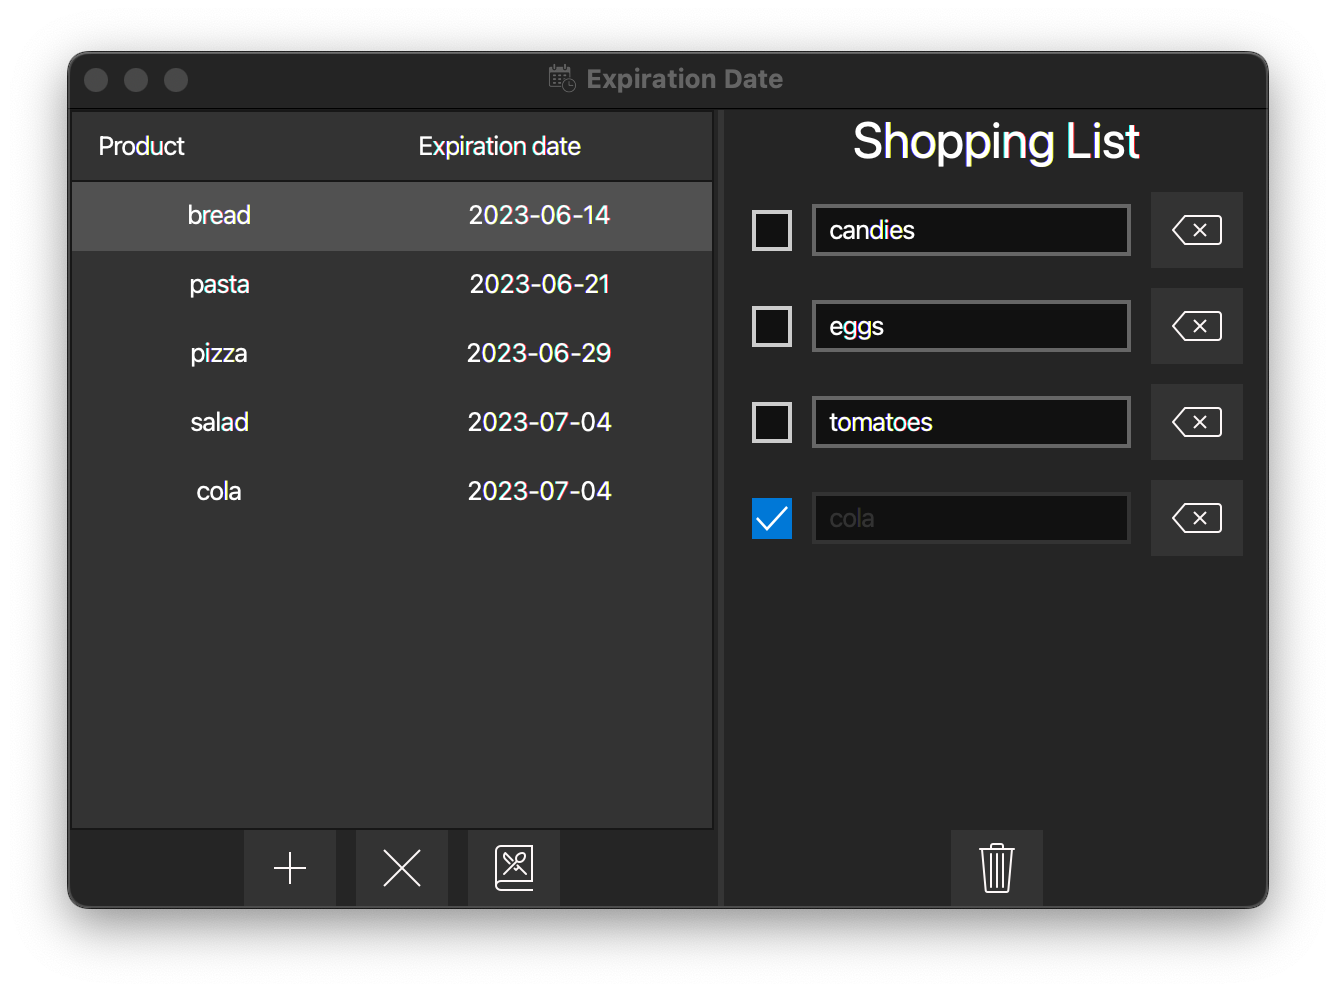
\includegraphics[width=\linewidth]{images/main-view.png}
    \caption{Finestra per la gestione di dispensa e lista della spesa.}
    \label{fig:mainview}
\end{figure}

La schermata per la gestione della dispensa e della lista della spesa si divide in due parti:

\begin{itemize}
  \item la parte di sinistra permette di aggiungere prodotti alla dispensa, eliminare prodotti dalla dispensa, modificare i dati di un prodotto o passare alla schermata delle ricette
  \begin{itemize}
    \item nel caso si desideri modificare i dati di un prodotto comparirà una schermata apposita per la modifica

    \begin{figure}[H]
        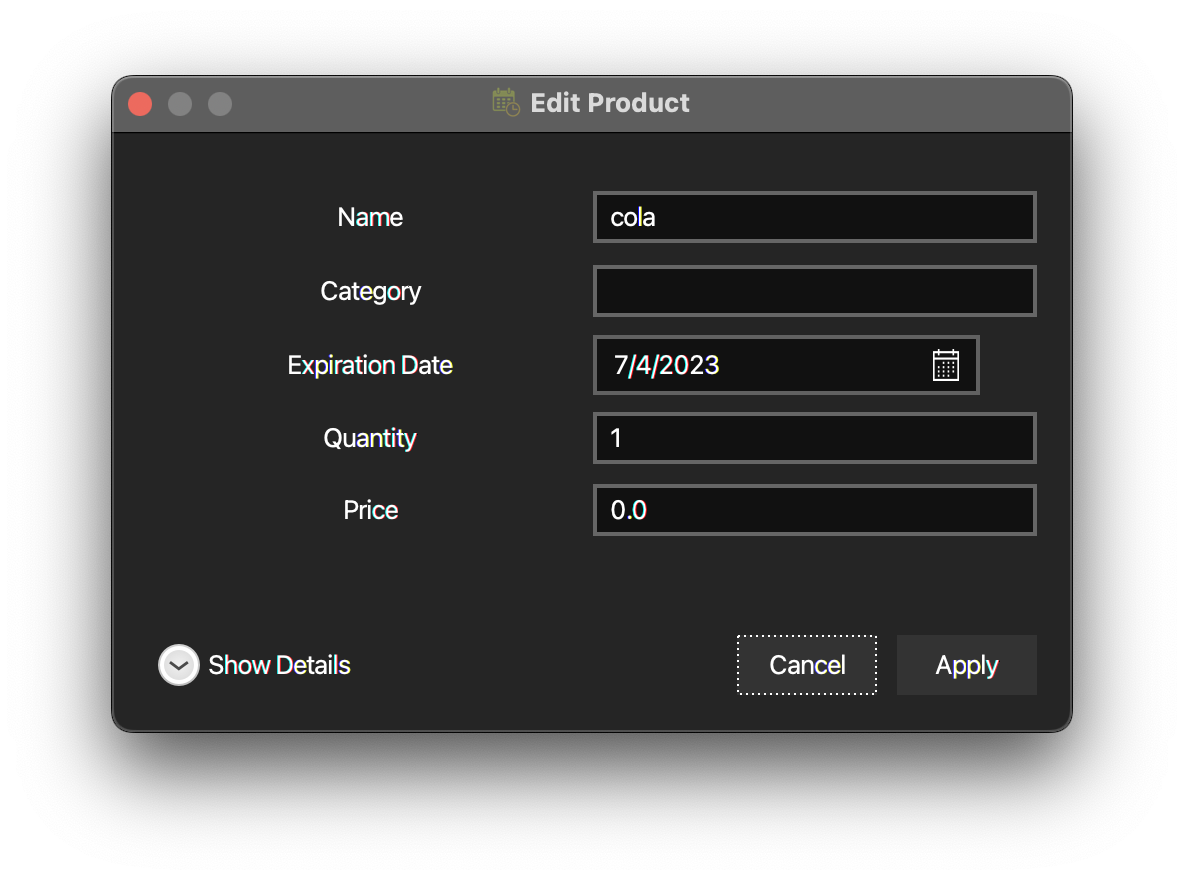
\includegraphics[width=\linewidth]{images/edit-product.png}
        \caption{Finestra per la modifica dei dati del prodotto.}
        \label{fig:editproduct}
    \end{figure}

  \end{itemize}
  \item la parte di destra permette di aggiungere prodotti alla lista della spesa, eliminare prodotti dalla lista della spesa, contrassegnare un prodotto della lista della spesa come "acquistato" (e aggiungerlo in automatico alla dispensa) e rimuovere tutti i prodotti contrassegnati come acquistati
\end{itemize}

\newpage

La schermata per la gestione delle ricette permette di navigare tra le ricette con le apposite frecce, aggiungere una ricetta, rimuovere una ricetta, modificare i dati di una ricetta, importare ed esportare liste di ricette.

\begin{figure}[H]
    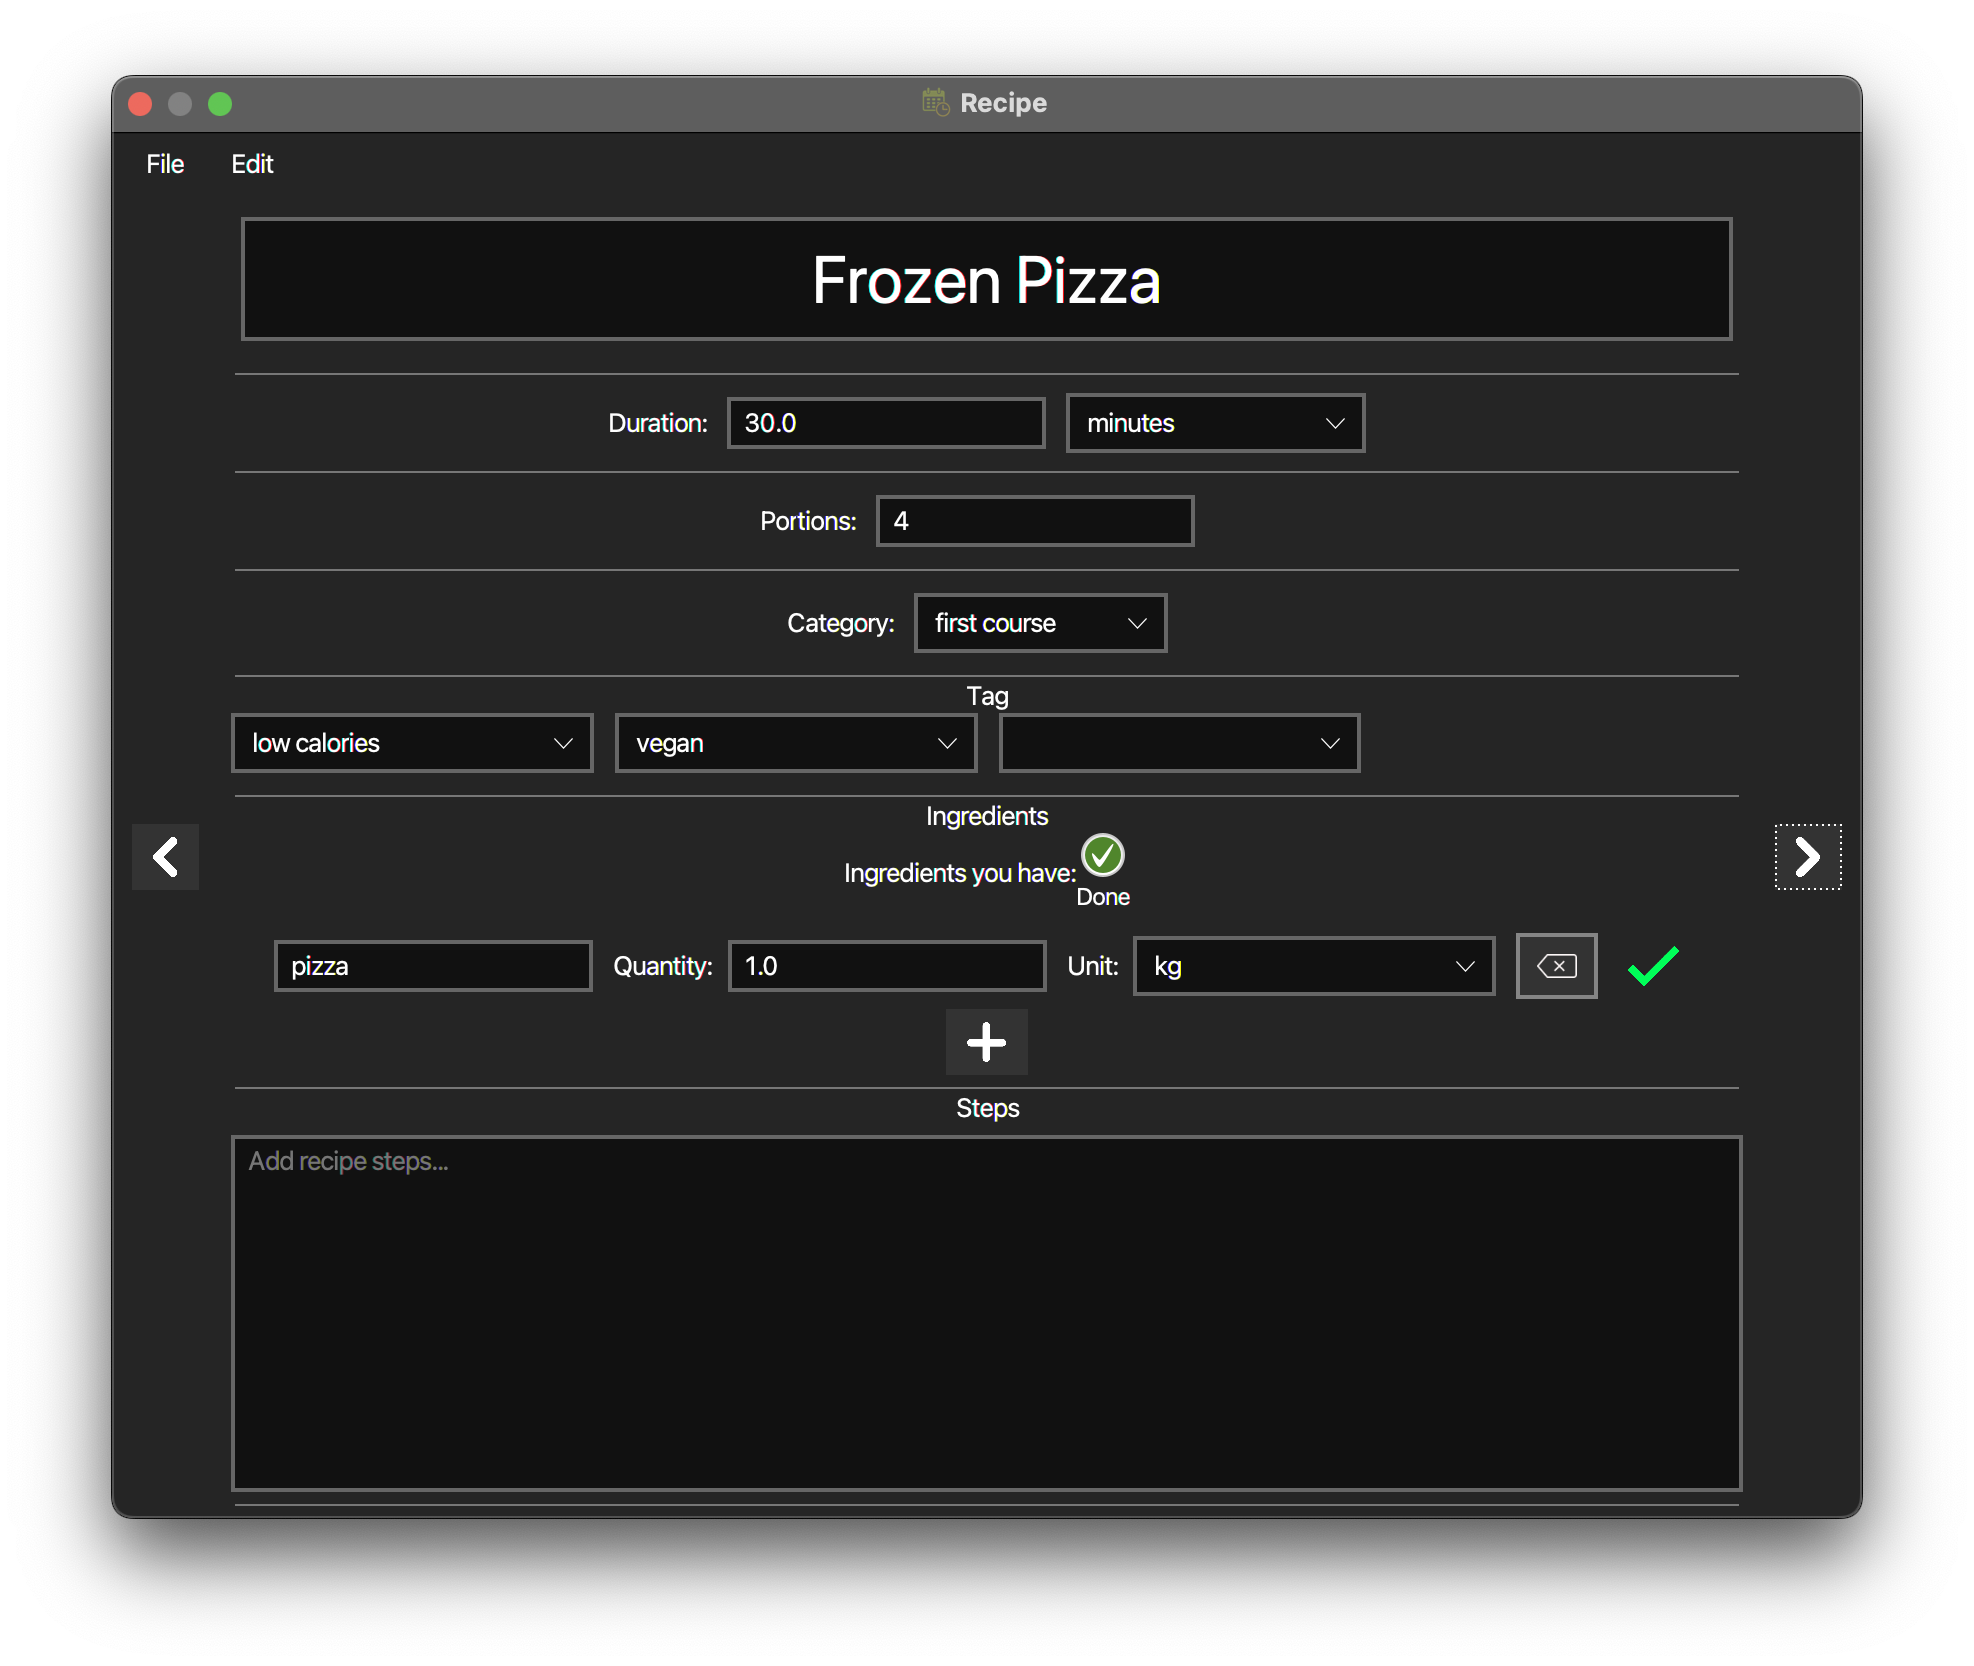
\includegraphics[width=\linewidth]{images/recipe-view.png}
    \caption{Finestra per la gestione delle ricette.}
    \label{fig:recipeview}
\end{figure}


\chapter{UML}

I diagrammi UML permettono di descrivere graficamente l'applicazione sotto vari punti di vista, garantendo la comprensione del funzionamento del software, delle esigenze che esso soddisfa e delle relazioni che intercorrono fra i suoi componenti.

Esistono diverse tipologie di diagrammi UML, quelle riportate nel presente documento sono:
\begin{itemize}
    \item diagramma dei casi d'uso
    \item diagramma delle attività
    \item diagramma degli stati
    \item diagramma delle classi
    \item diagramma di sequenza
\end{itemize}

Per ciascuno di essi verrà offerta una breve panoramica che includerà:
\begin{itemize}
    \item significato del diagramma 
    \item contesto in cui viene utilizzato
    \item funzionalità specifica dell'applicazione che viene descritta
    \item eventuali precisazioni/omissioni all'interno del diagramma e motivazione delle stesse
\end{itemize}

\section{Use case diagram}

\begin{figure}[H]
    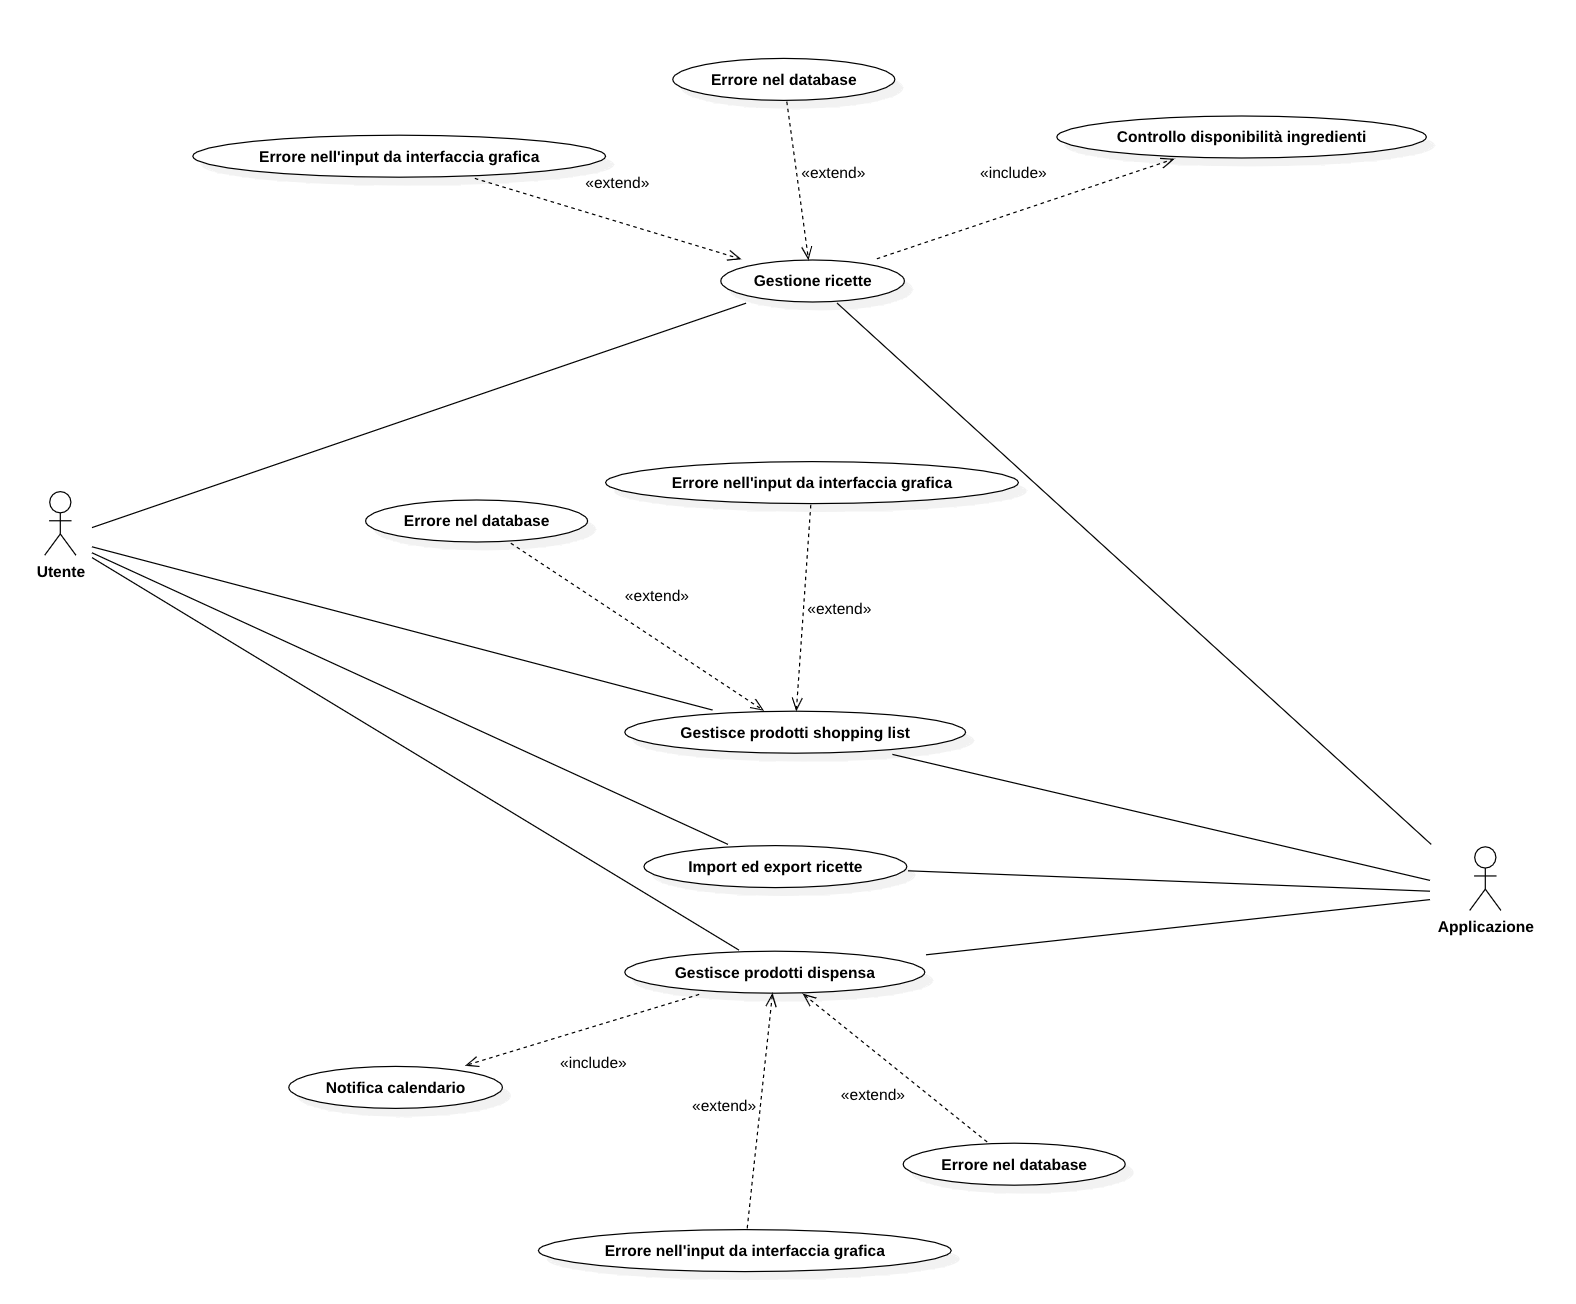
\includegraphics[width=\linewidth]{images/use-case.png}
    \caption{Diagramma dei casi d'uso.}
    \label{fig:usecase}
\end{figure}

Lo use case diagram permette di identificare gli attori che interagiscono col sistema e le attività che essi possono svolgere. Lo scopo è descrivere le principali funzionalità del software.

\newpage

\section{Activity diagram}

L'activity diagram consente di specificare come il sistema realizzerà le funzionalità mostrate nello use case. Lo scopo è connettere tra loro azioni di alto livello per rappresentare un processo che viene svolto nel sistema. Per una migliore comprensione del funzionamento, nei diagrammi seguenti si è scelto di non modellare i casi di errore del database e dell'interfaccia grafica. 

\subsection{Activity diagram della dispensa}

In questo diagramma viene mostrato il processo relativo all'interazione fra l'utente e l'applicazione per la gestione della dispensa. 

\begin{figure}[H]
    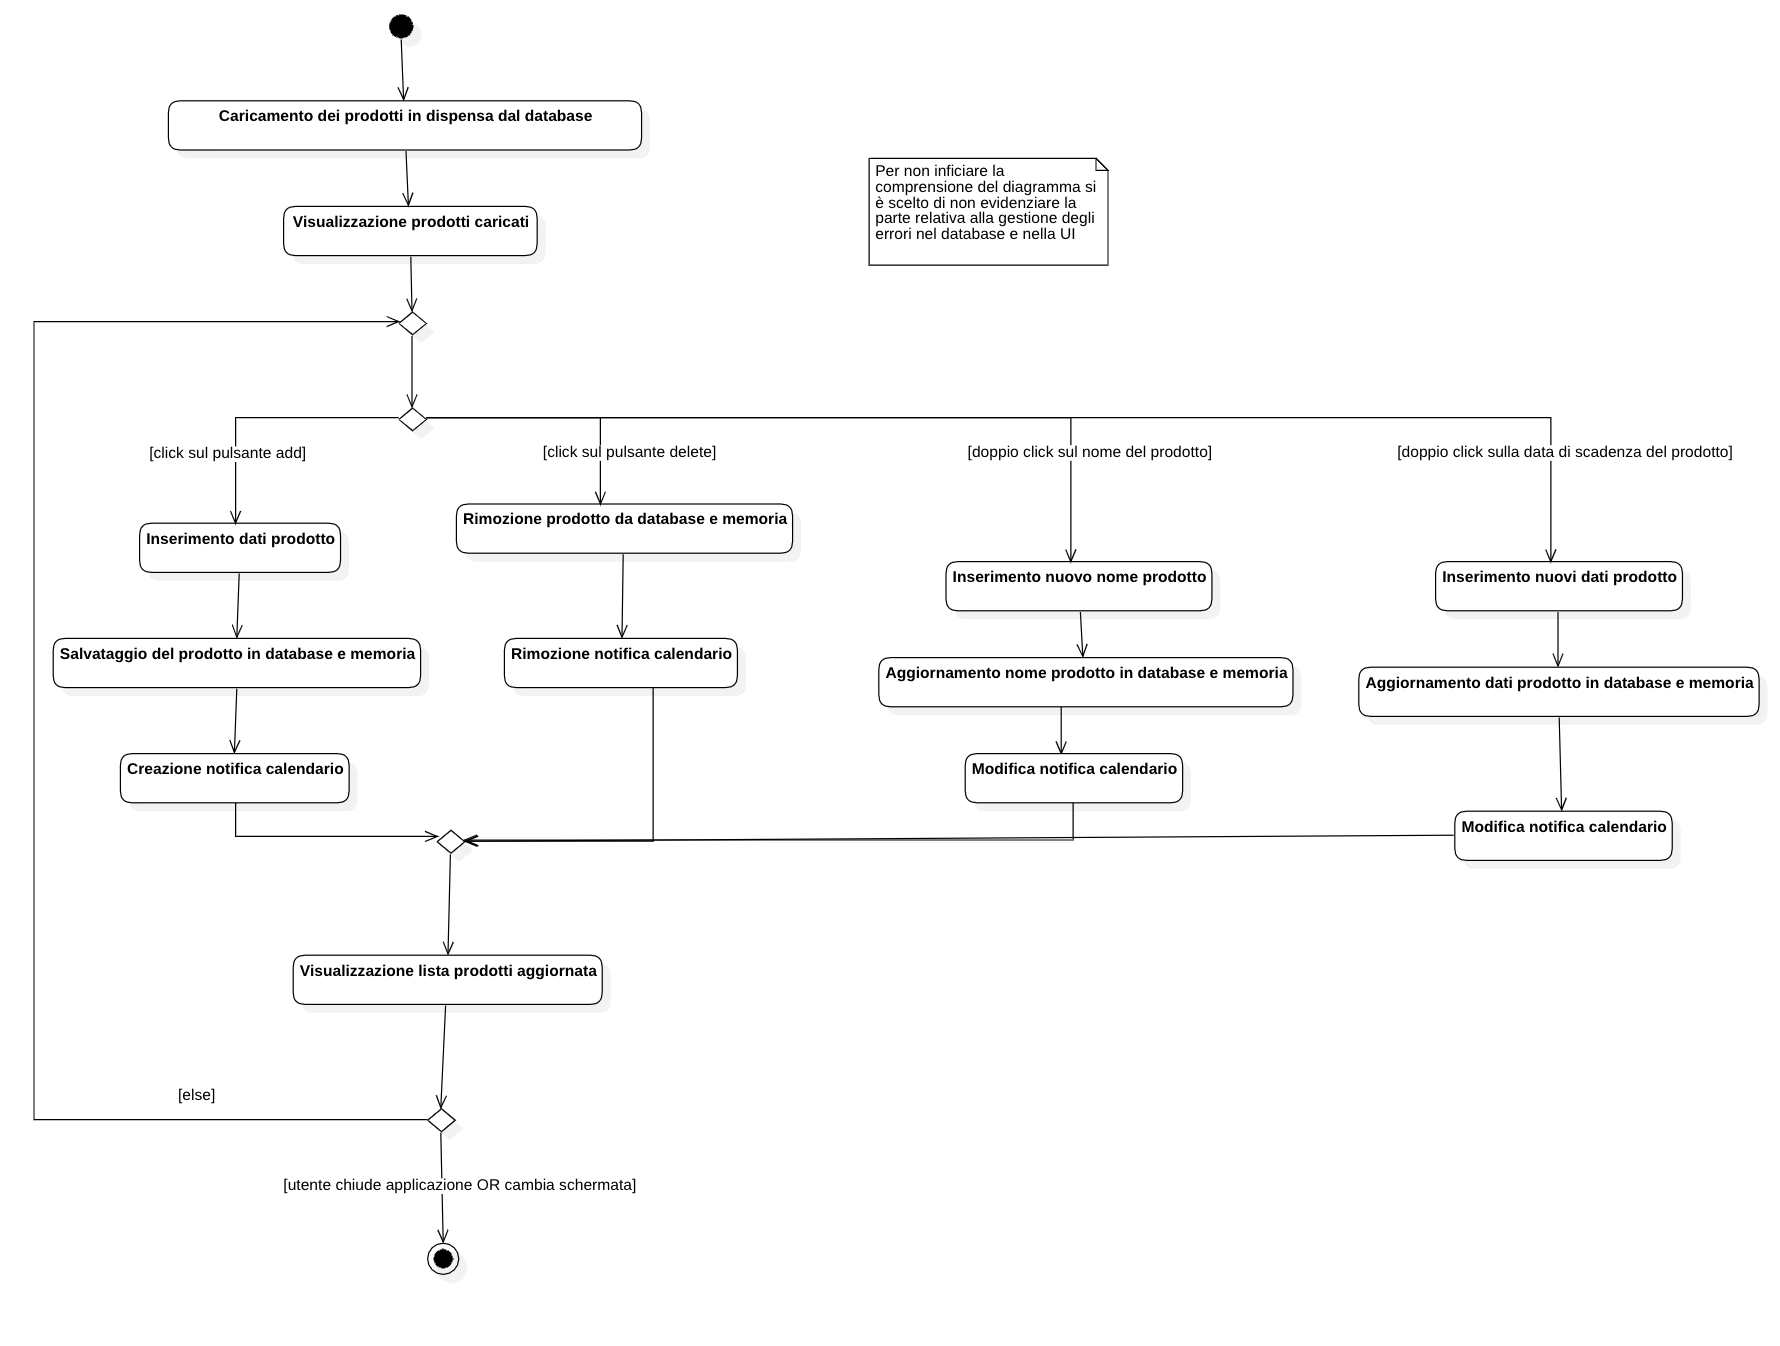
\includegraphics[width=\linewidth]{images/activity-pantry.png}
    \caption{Diagramma delle attività della dispensa.}
    \label{fig:actpantry}
\end{figure}

\newpage

\subsection{Activity diagram della lista della spesa}

In questo diagramma viene mostrato il processo relativo all'interazione fra l'utente e l'applicazione per la gestione della lista della spesa.

\begin{figure}[H]
    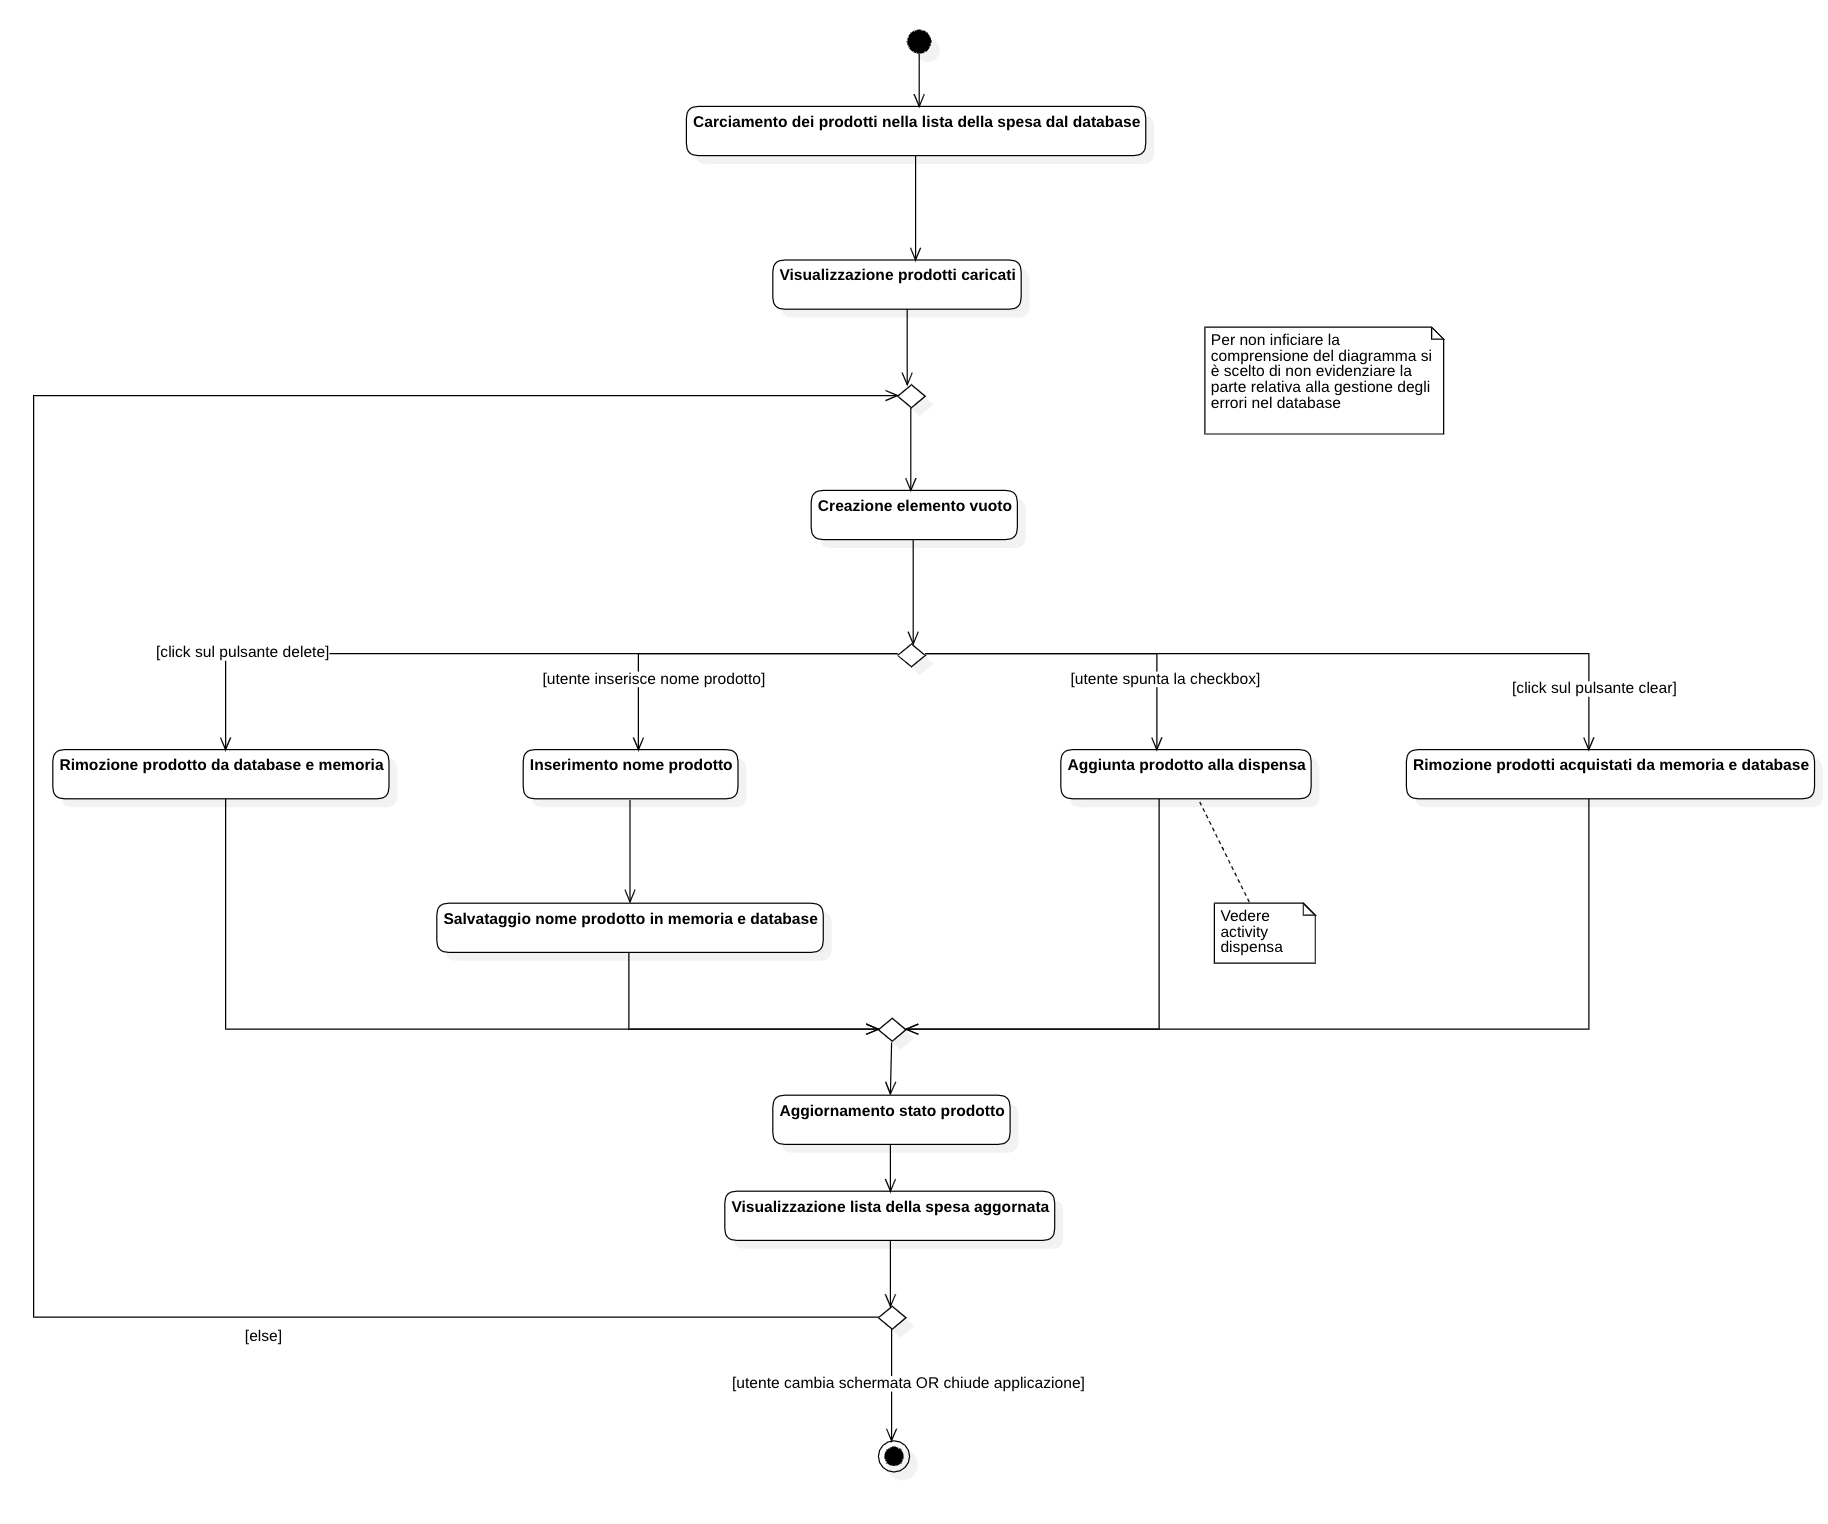
\includegraphics[width=\linewidth]{images/activity-shopping-list.png}
    \caption{Diagramma delle attività della lista della spesa.}
    \label{fig:actshoplist}
\end{figure}

\newpage

\subsection{Activity diagram delle ricette}

In questo diagramma viene mostrato il processo relativo all'interazione fra l'utente e l'applicazione per la gestione delle ricette, inclusa la possibilità di importare ed esportare ricette.

\begin{figure}[H]
    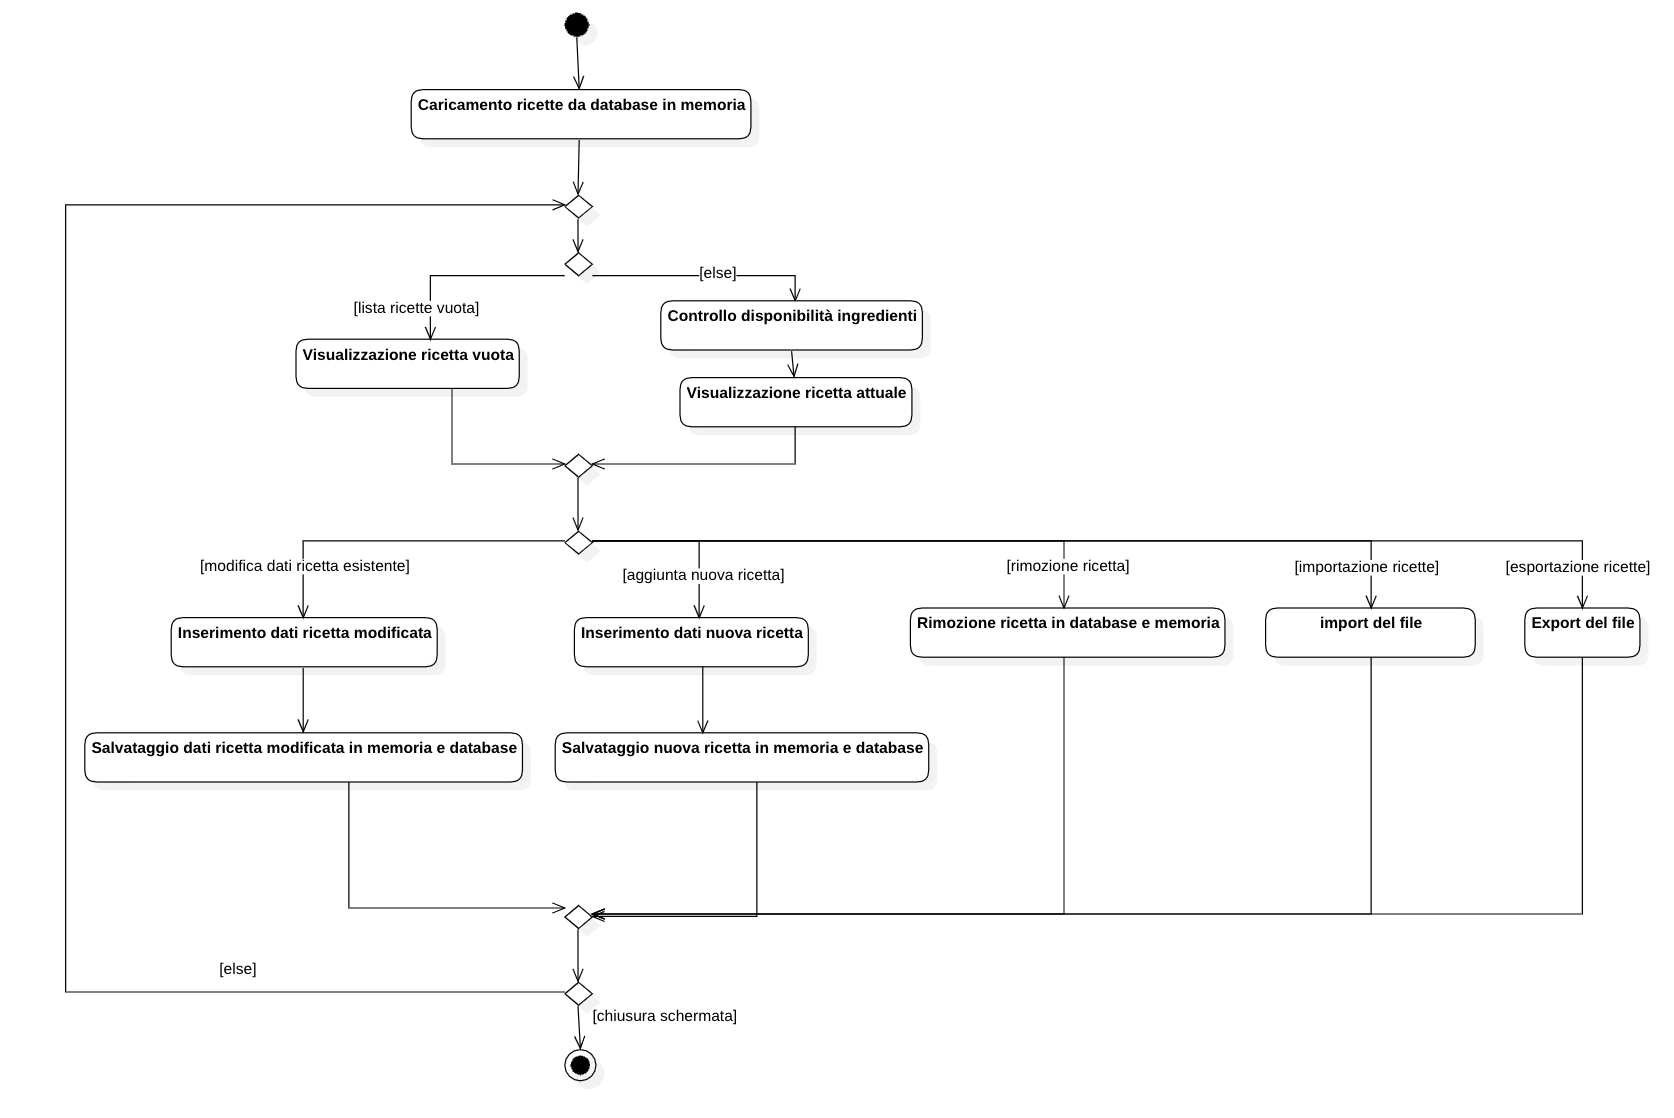
\includegraphics[width=\linewidth]{images/activity-recipe.png}
    \caption{Diagramma delle attività delle ricette.}
    \label{fig:actrecipe}
\end{figure}

\newpage

\section{State diagram}

Lo state diagram permette di modellare gli stati in cui si trova un oggetto e gli eventi che causano le transizioni fra gli stati. 

\subsection{State diagram della ricetta}

In questo diagramma vengono mostrati gli stati in cui si può trovare una ricetta in base alla presenza, e alla disponibilità, degli ingredienti.

\begin{figure}[H]
    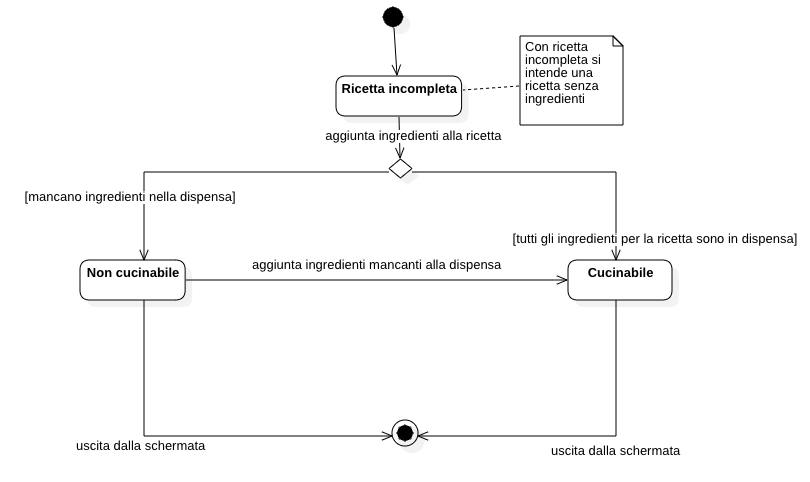
\includegraphics[width=\linewidth]{images/state-recipe.png}
    \caption{Diagramma degli stati della ricetta.}
    \label{fig:staterecipe}
\end{figure}

\newpage

\subsection{State diagram della lista della spesa}

In questo diagramma vengono mostrati gli stati in cui si può trovare un prodotto presente nella lista della spesa.

\begin{figure}[H]
    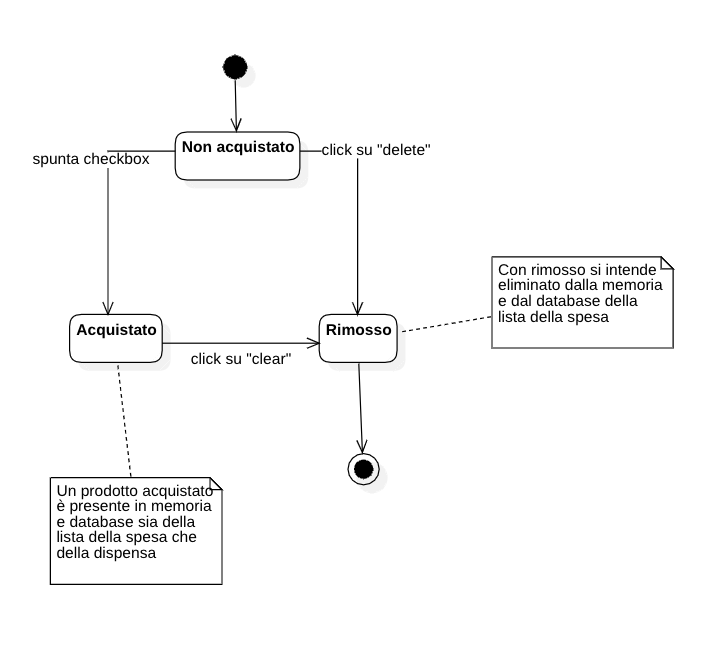
\includegraphics[width=\linewidth]{images/state-shopping-list.png}
    \caption{Diagramma degli stati della lista della spesa.}
    \label{fig:stateshoplist}
\end{figure}

\newpage

\section{Class diagram}

Il class diagram permette di descrivere i tipi di oggetti presenti nel sistema e le relazioni statiche che intercorrono tra di essi. Esso descrive inoltre gli attributi e i metodi di ogni classe, oltre ai vincoli che si applicano nel collegamento tra gli oggetti.

\begin{figure}[H]
    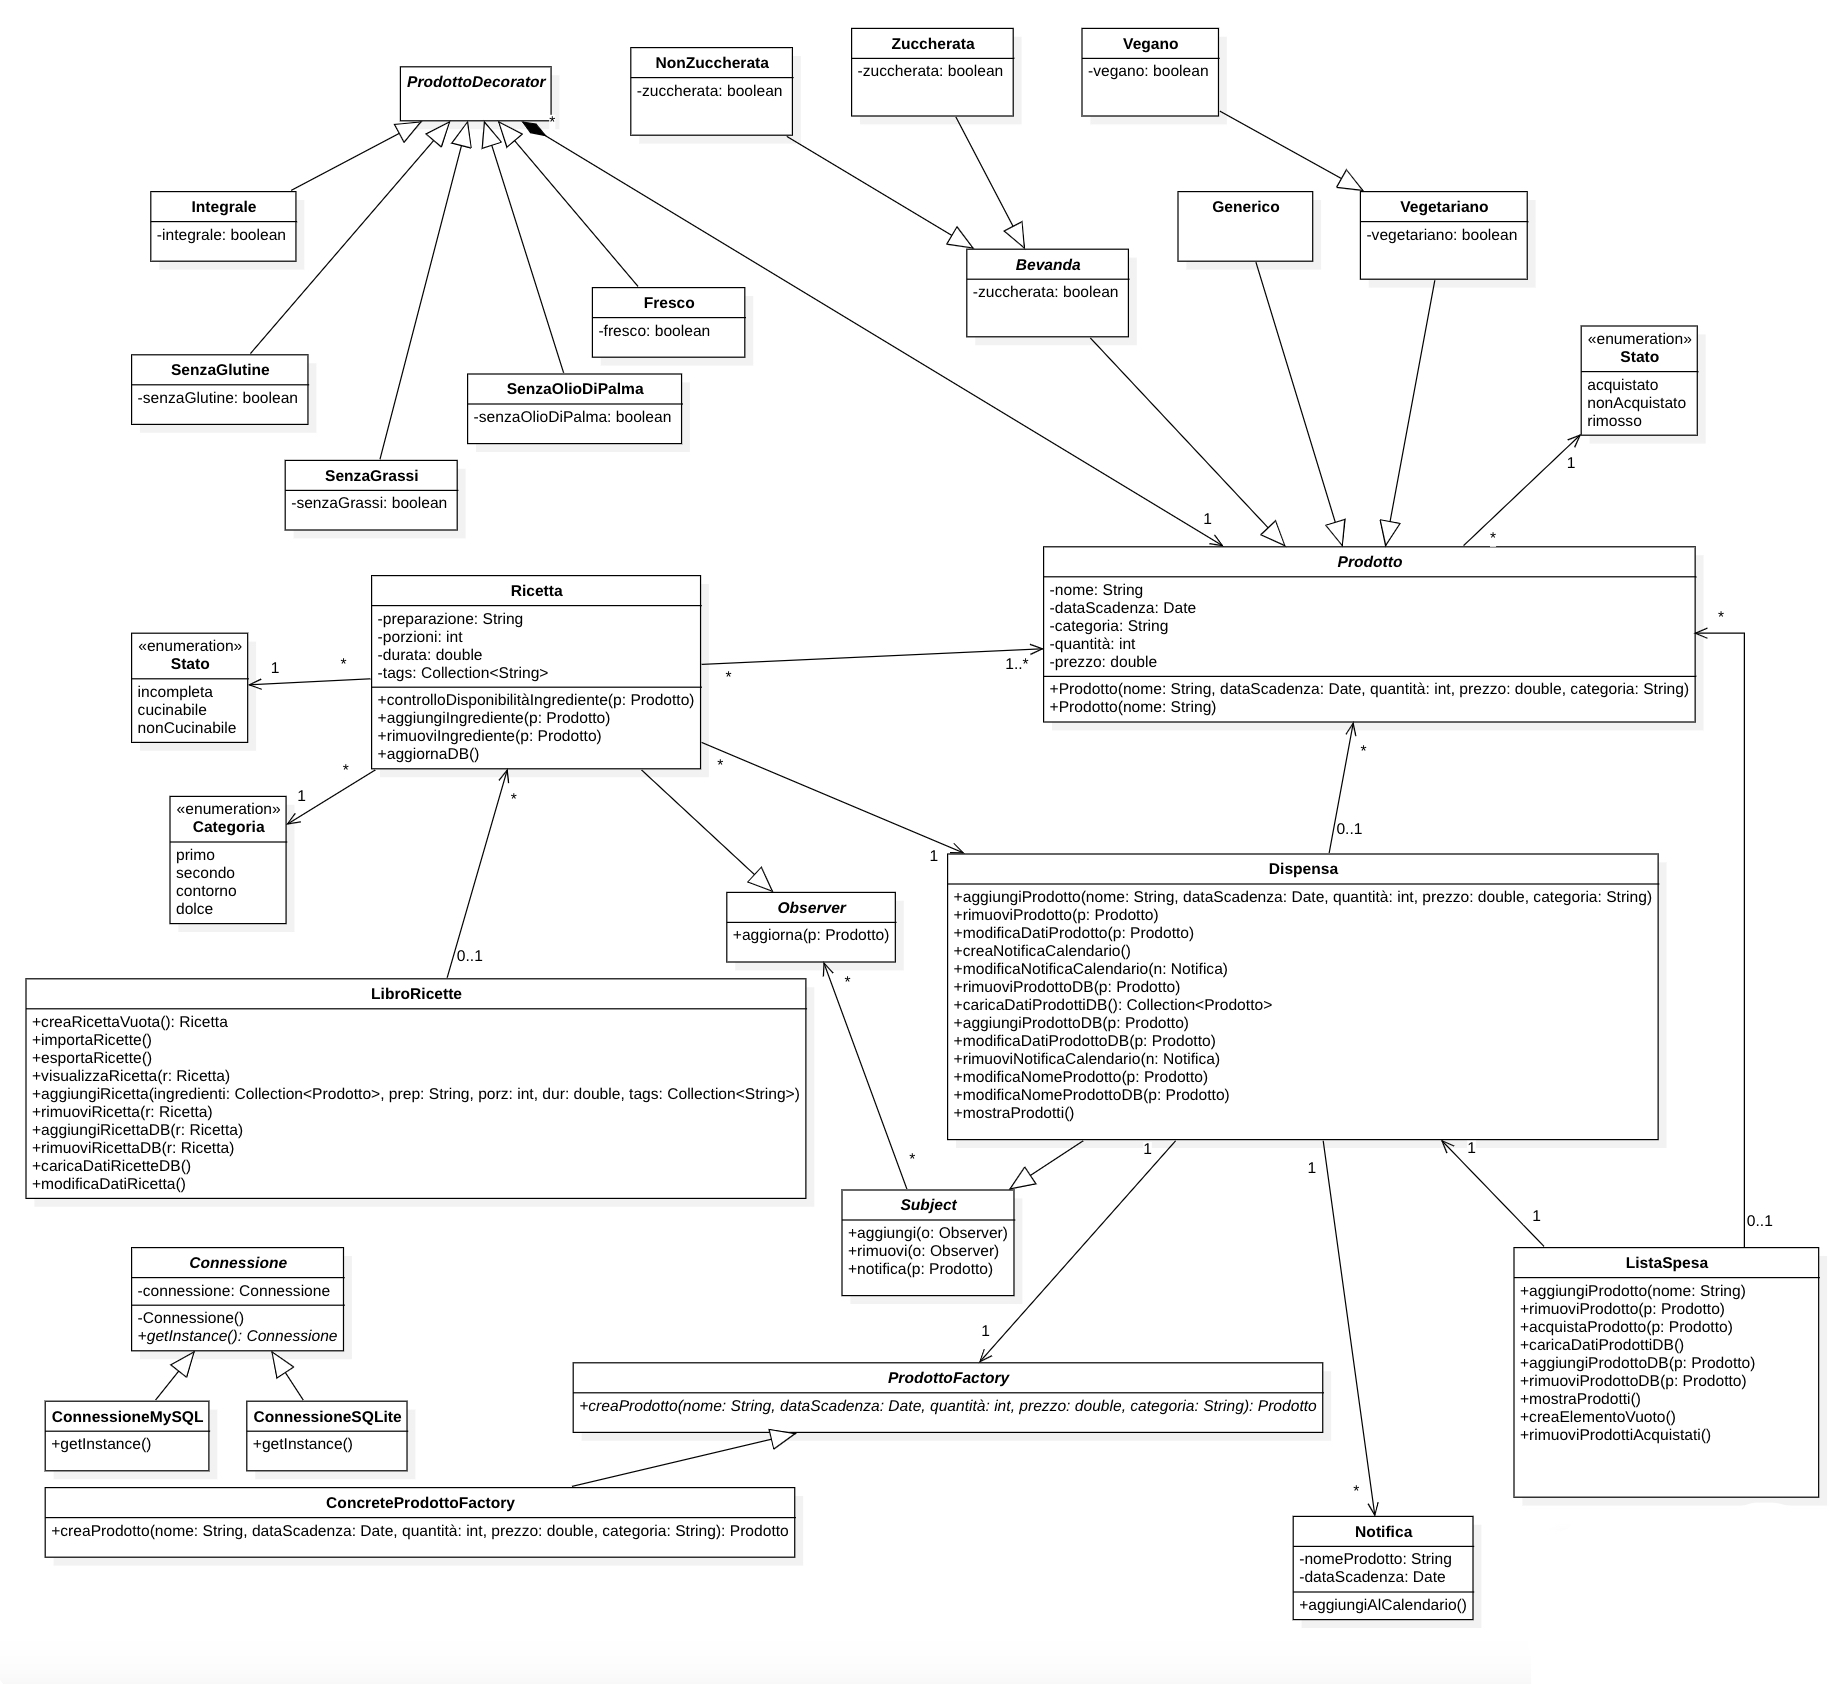
\includegraphics[width=\linewidth]{images/class.jpeg}
    \caption{Diagramma delle classi.}
    \label{fig:classdiagram}
\end{figure}

Per non complicare ulteriormente il diagramma si è scelto di non rappresentare la parte relativa all'interfaccia grafica. I design pattern applicati verranno spiegati nella sezione corrispondente.

\newpage

\section{Sequence diagram}

Il sequence diagram serve per descrivere singoli scenari dell'applicazioni. Lo scopo è mostrare come il sistema svolge le proprie funzioni. Per una migliore comprensione del funzionamento, nei diagrammi seguenti si è scelto di non modellare i casi di errore del database e dell'interfaccia grafica. 

Gli elementi principali di un sequence diagram, usati in tutti gli esempi successivi, comprendono:
\begin{itemize}
\item lifeline: rappresenta l'esistenza di un'entità in un dato istante della sequenza (utile quando un'entità è creata o eliminata durante una sequenza)
\item entità: attore/parte che interagisce con altri attori/parti; sono dotate di un nome ed eventualmente di una classe
\item messaggi: segnali che un partecipante (un'entità) invia ad un altro partecipante oppure provenienti da agenti esterni; possono essere specificati parametri, tipo del valore di ritorno
\item frammenti: operatori usati per modellare varie strutture di controllo, permettono di rappresentare molteplici flussi di esecuzione in maniera compatta e precisa
\item Esempi di frammenti utilizzati nei diagrammi seguenti
\begin{itemize}
    \item alt: rappresenta un \textit{if} con più condizioni (o \textit{guardie})
    \item opt: rappresenta un \textit{if} con una sola condizione
    \item loop: usato per modellare i cicli
\end{itemize}
\item Esempi di altri frammenti, usati per modellare l'ordine di esecuzione (seq, strict, par, critical) o l'occorrenza dei messaggi (ignore, consider, assert, neg)
\begin{itemize}
\item break: simboleggia la conclusione anticipata di un ciclo rispetto alla sua canonica esecuzione, spesso in seguito alla rilevazione di un'eccezione
\item seq: rappresenta l'ordinamento di default (ordinamento debole)
\item strict: rappresenta un ordinamento forte
\item par: permette di separare l'ordine degli operandi rendendoli indipendenti l'uno dall'altro (e potenzialmente eseguibili contemporaneamente)
\item critical: definisce un'area atomica nell'interazione, garantendo che essa non venga interrotta da eventi inaspettati
\item ignore: indica che il messaggio ricevuto è irrilevante
\item consider: indica che il messaggio ricevuto è di particolare importanza per l'interazione che si sta analizzando
\item assert: usato per definire situazioni che devono avvenire
\item neg: permette di modellare un'interazione invalida, come ad esempio i messaggi di errore
\end{itemize}
\end{itemize}

\subsection{Sequence diagram della dispensa}

\begin{figure}[H]
    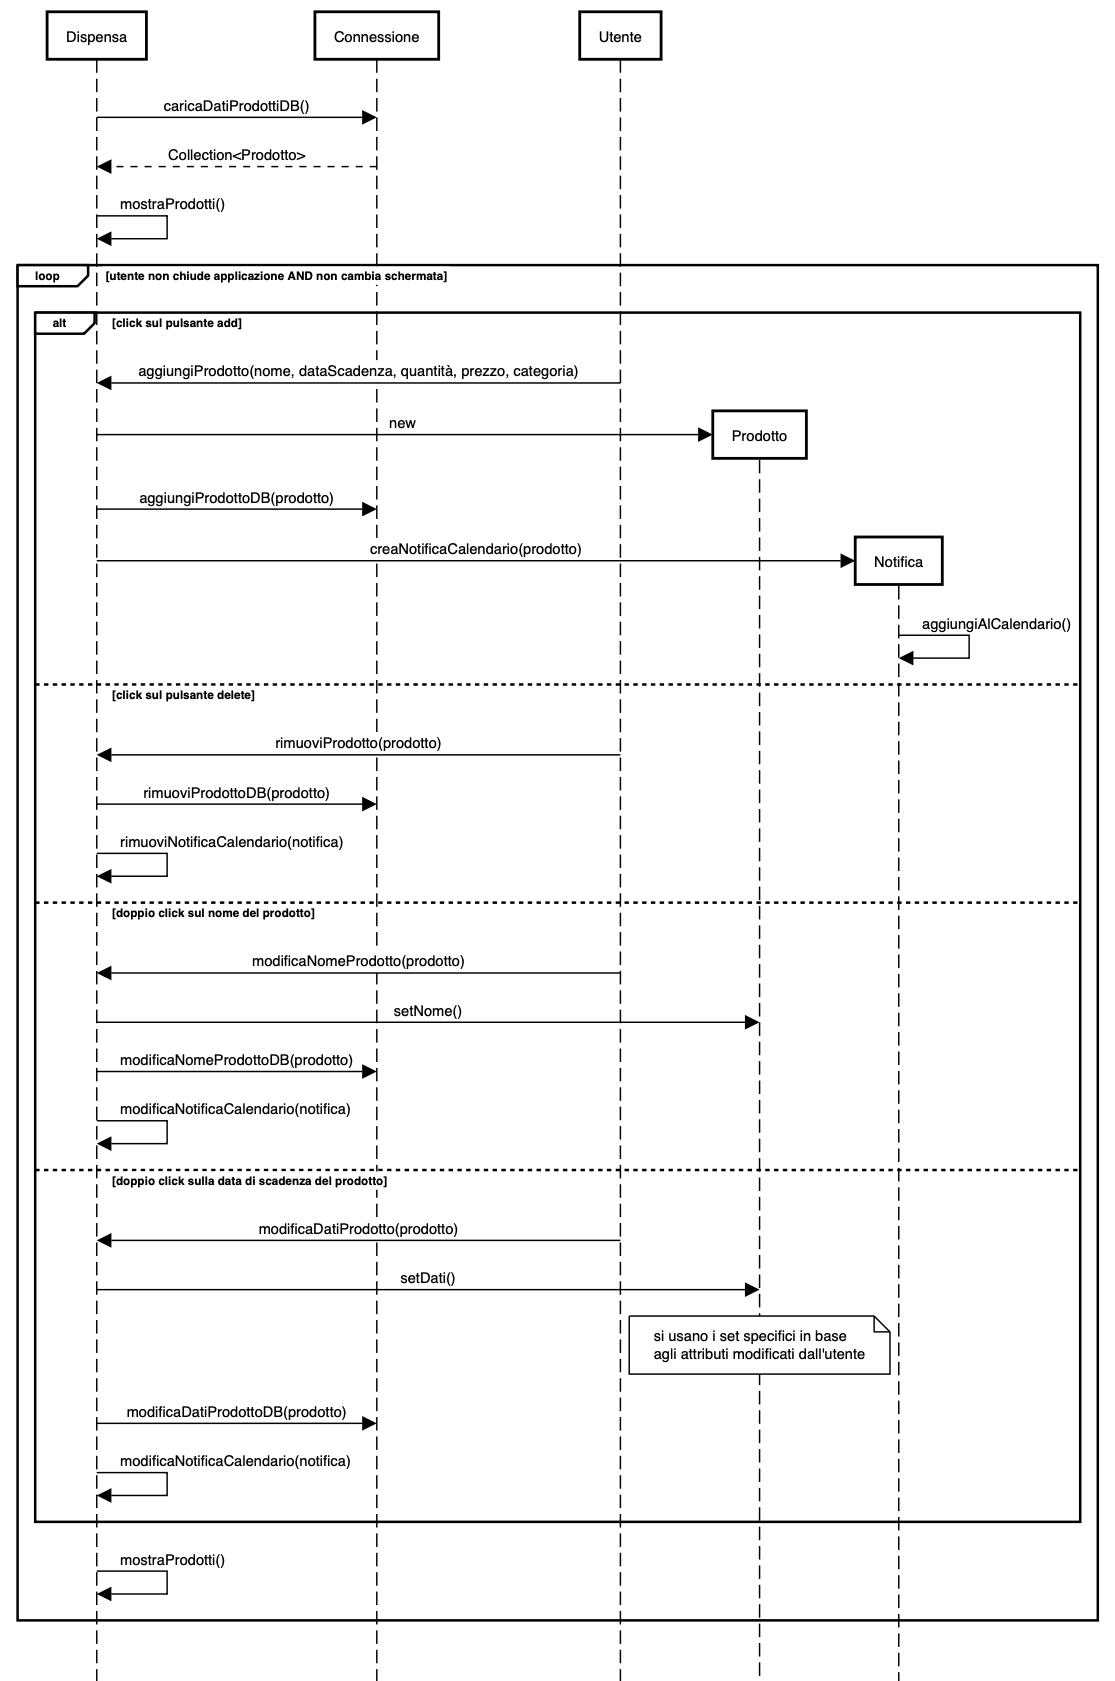
\includegraphics[width=\linewidth]{images/sequence-pantry.png}
    \caption{Diagramma di sequenza della dispensa}
    \label{fig:seqpantry}
\end{figure}

\subsection{Sequence diagram della lista della spesa}

\begin{figure}[H]
    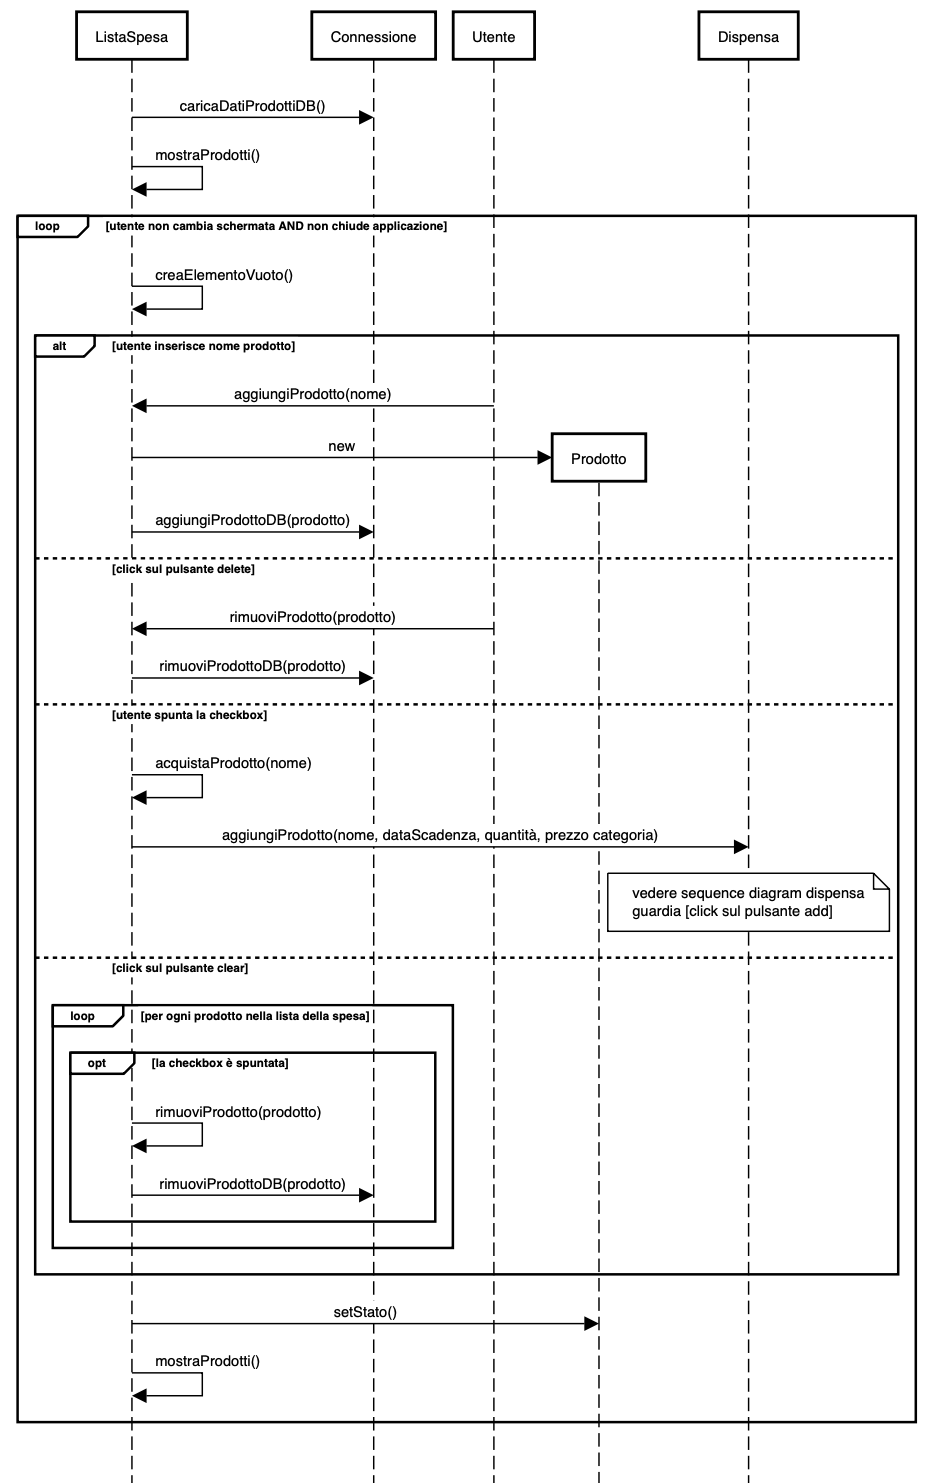
\includegraphics[width=\linewidth]{images/sequence-shopping-list.png}
    \caption{Diagramma di sequenza della lista della spesa}
    \label{fig:seqshoplist}
\end{figure}

\subsection{Sequence diagram delle ricette}

\begin{figure}[H]
    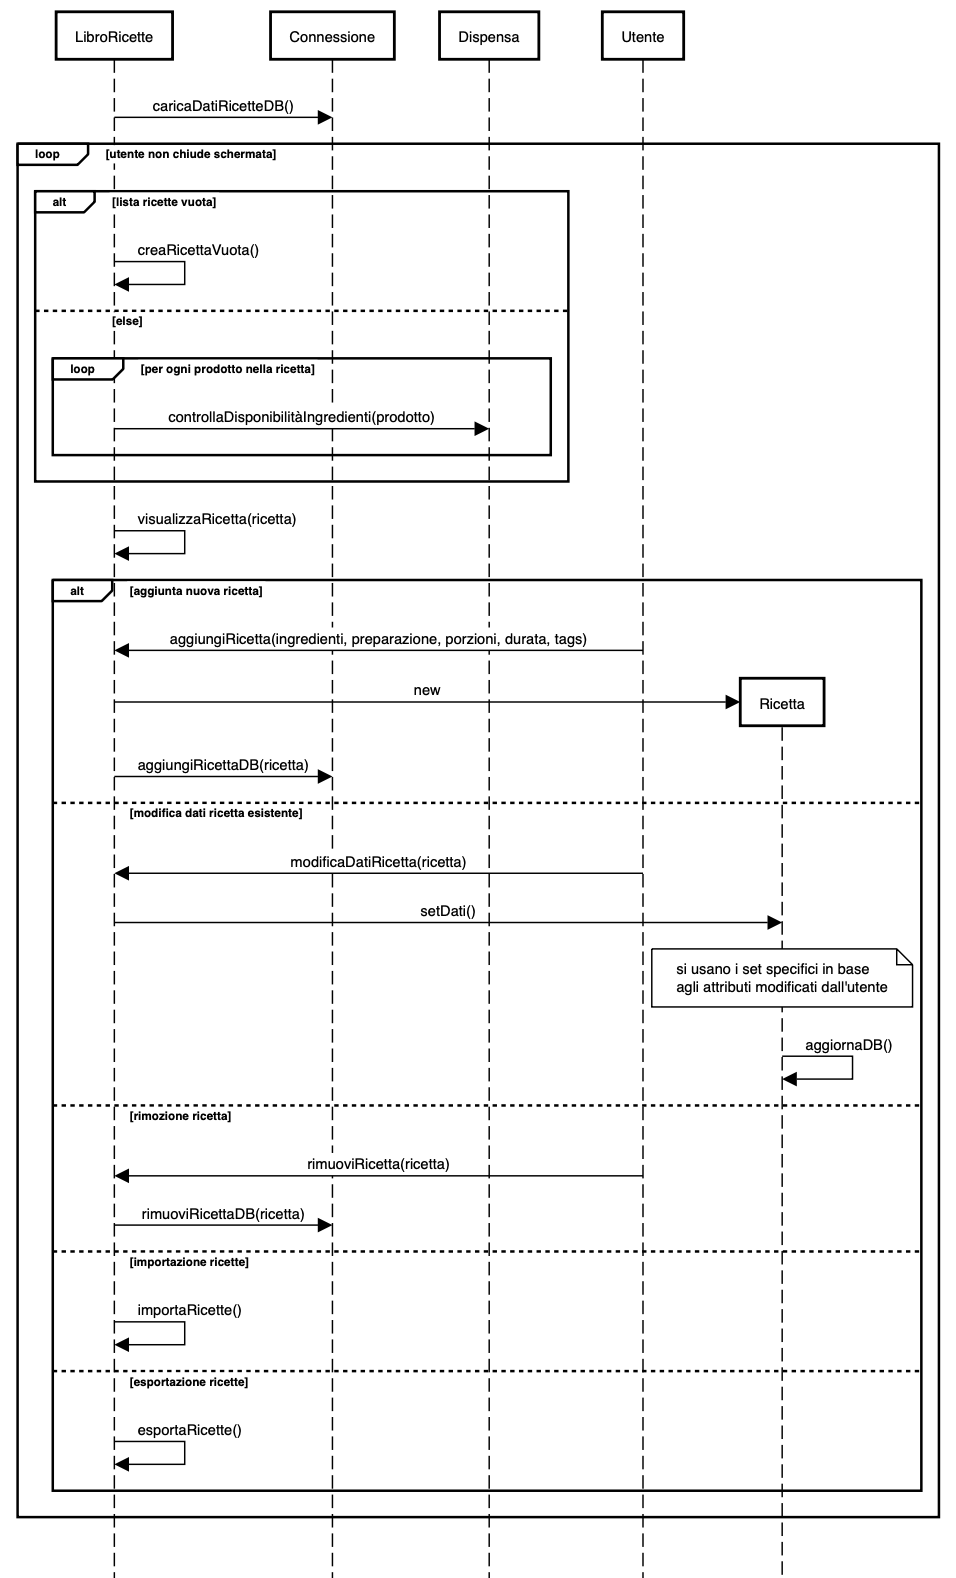
\includegraphics[width=\linewidth]{images/sequence-recipe.png}
    \caption{Diagramma di sequenza delle ricette}
    \label{fig:seqrecipe}
\end{figure}

Si noti che, per evitare sovrapposizioni nel diagramma che ne avrebbero resa più difficile la comprensione, il metodo \inlinecode{Java}{creaRicettaVuota()} (che si limita a mostrare dei campi di testo vuoti all'utente tramite l'interfaccia grafica) non crea un oggetto di tipo Ricetta (come invece avviene nel caso del metodo \\ \inlinecode{Java}{aggiungiRicetta(ingredienti, preparazione, porzioni, durata, tags)} in cui la ricetta creata presenta valori non nulli nei propri attributi).



\chapter{Design Pattern}

L'applicazione implementa diversi Design Pattern per garantire una manutenzione più agevole del codice, rendere il software più modulare semplificando l'aggiunta di nuove funzionalità, consentire la parallelizzazione dello sviluppo.

\section{Factory}

Il design pattern Factory ha il compito di occuparsi della creazione dei prodotti. L'utilizzo di questo design permette di evitare di programmare verso le implementazioni concrete, favorendo la programmazione verso le interfacce. Senza di esso, quando in futuro dovranno essere apportare modifiche o estensioni, sarebbe necessario riaprire il codice e cambiarlo di conseguenza (violando quindi l'open-closed principle). Incapsulare la creazione dei prodotti in una apposita classe permette di evitare questo scenario, oltre a facilitare la manutenzione e l'aggiornamento dell'applicazione: le modifiche sono infatti localizzate unicamente nella classe Factory, mentre in mancanza di essa sarebbe necessario cambiare manualmente tutti i punti del codice in cui c'è un "new" di un prodotto. L'utilizzo del design pattern Factory rispetta inoltre il dependency inversion principle. 

\begin{lstlisting}
  // Beverage.java
  public abstract class Beverage extends Product{
    boolean sweet;
    public Beverage(String name, LocalDate expirationDate, 
    int quantity, double price, String category){
      super(name, expirationDate, quantity, price, category);
    }
  }
  // SweetBeverage.java
  public class SweetBeverage extends Beverage{
	  public SweetBeverage(String name, LocalDate expirationDate,
      int quantity, double price, String category) {
		  super(name, expirationDate, quantity, price, category);
		  sweet = true;
	  }
  }

  
  // ProductFactory.java
  public abstract class ProductFactory {
	public abstract Product createProduct(String name, 
    LocalDate expirationDate, int quantity, double price,
	String category);
  }
  // ConcreteProductFactory.java
  public class ConcreteProductFactory extends ProductFactory{
    @Override
    public Product createProduct(String name, LocalDate expirationDate,
    int quantity, double price, String category) {
      if("sweet beverage".equals(category)){
        return new SweetBeverage(name, expirationDate, quantity,
         price, category);
      } else if("non sweet beverage".equals(category)){
        return new NonSweetBeverage(name, expirationDate, quantity,
         price, category);
      } else if("generic product".equals(category)){
        return new GenericProduct(name, expirationDate, quantity,
         price, category);
      } else if("vegetarian product".equals(category)){
        return new VegetarianProduct(name, expirationDate, quantity,
         price, category);
      } else if("vegan product".equals(category)){
        return new VeganProduct(name, expirationDate, quantity,
         price, category);
      } else return null;
    }
  }
\end{lstlisting}

Si noti come, nella classe \inlinecode{Java}{ConcreteProductFactory}, sia stata utilizzata una tecnica di defensive programming per evitare una \inlinecode{Java}{NullPointerException}.

\section{Iterator}

Il design pattern Iterator consente di incapsulare il modo di iterare su una collezione di elementi, nascondendo l'implementazione interna della struttura dati e fornendo un modo unico per navigare attraverso tipi di dato diversi (a patto che implementino l'iterator). Questo design pattern permette di programmare verso le interfacce, disaccoppiando il codice che si occupa di svolgere l'iterazione dalle classi concrete su cui itera. Java ha un proprio iterator e la maggior parte delle collezioni di oggetti implementa la sua interfaccia, pertanto è sufficiente utilizzare i metodi già offerti dalla libreria standard.

\begin{lstlisting}
  public class Recipe implements Observer{
    List<Product> ingredients;
    // other attributes and methods of the class
    public void checkIngredientAvailability(Product p){
      for(Iterator<Product> iterator = ingredients.iterator();
      iterator.hasNext();){  
          Product product = iterator.next();
          // method implementation  
        }
    }
  }
\end{lstlisting}

\section{Observer}

Il design pattern Observer permette agli oggetti di essere notificati quando qualcosa di loro interesse cambia. Questo design pattern permette di programmare verso le interfacce, svincolandosi dalle implementazioni concrete ed evitando di violare l'open-closed principle tramite l'incapsulamento di ciò che varia e la sua separazione da ciò che non varia. Applicando questo design pattern si ottiene inoltre una riduzione dell'accoppiamento tra le classi che vengono osservate e le classi che osservano. Per esempio, le ricette possono osservare la dispensa in modo da essere notificate quando un prodotto viene aggiunto o rimosso e poter aggiornare la disponibilità degli ingredienti. 

\begin{lstlisting}
  public class Pantry implements Subject {
    List<Observer> observers = new ArrayList<>();
    ProductFactory productFactory;
    // other attributes and methods of the class
    public void addProduct(String name, LocalDate expirationDate, int quantity, double price, String category){
      Product p = productFactory.createProduct(name, expirationDate, quantity, price, category);
      // method implementation
      notify(p);
    }
    public void notify(Product p){
      for(Iterator<Observer> iterator = observers.iterator(); iterator.hasNext()){
        Observer observer = iterator.next();
        observer.update(p);
      }
    }
  }
  public class Recipe implements Observer {
    // attributes and methods of the class
    public void update(Product p){
      checkIngredientAvailability(p);
    }
  }
\end{lstlisting}

\section{Singleton}

Per la connessione al database si utilizza il design Pattern Singleton in modo da garantire l'unicità dell'istanza creata e un punto di accesso globale a questa istanza. Applicando questo design pattern si rispetta il dependency inversion principle, poiché si dipende da una interfaccia per la connessione al database: in questo modo modifiche nell'implementazione concreta del database non impatteranno sulle classi che ne fanno uso. Inoltre rispetta anche l'open-closed principle, in quanto per aggiungere un nuovo database basterà creare una nuova classe che implementi l'interfaccia senza dover modificare il codice relativo alle implementazioni precedenti.

\section{Decorator}

Il design pattern Decorator permette di aggiungere funzionalità (metodi o attributi) agli oggetti dinamicamente. Esso rispetta il principio di programmazione che afferma di favorire la composizione rispetto all'ereditarietà. In questo modo si hanno classi meno accoppiate tra loro, la manutenzione del codice è più semplice, il codice è più flessibile (estensioni future non violeranno l'open-closed principle). Nello specifico, il design pattern è applicato ai prodotti: in questo modo si potranno gestire agevolmente aggiunte e modifiche future, siano esse relative agli attributi dei prodotti o ad operazioni riservate solo a particolari tipologie di prodotti.

\begin{lstlisting}
  // Product.java
  public abstract class Product {
    String name;
    LocalDate expirationDate;
    String category;
    int quantity;
    double price;
    public Product(String name, LocalDate expirationDate,
    int quantity, double price, String category) {
      this.name = name;
      this.expirationDate = expirationDate;
      this.quantity = quantity;
      this.price = price;
      this.category = category;
    }
    // other methods' implementation
  }
  // GenericProduct.java
  public class GenericProduct extends Food{
	  public GenericProduct(String name, LocalDate expirationDate,
    int quantity, double price, String category) {
		  super(name, expirationDate, quantity, price, category);
	  }
  }
  // ProductDecorator.java
  public abstract class ProductDecorator {
    Product product;
    public ProductDecorator(Product product) {
      this.product = product;
    }
  }
  // FreshProductDecorator.java
  public class FreshProductDecorator extends ProductDecorator{
	  boolean fresh;
	  public FreshProductDecorator(Product product) {
		  super(product);
		  fresh = true;
	  }
  }
  // GlutenFreeProductDecorator.java
  public class GlutenFreeProductDecorator extends ProductDecorator{
    boolean glutenFree;
    public GlutenFreeProductDecorator(Product product) {
      super(product);
      glutenFree = true;
    }
  }
\end{lstlisting}

\chapter{ORM}

Per la parte relativa al database si è scelto di utilizzare la tecnica ORM (Object-Relational Mapping) per facilitare l'integrazione di database relazionali con software aderenti al paradigma della programmazione orientata agli oggetti. L'ORM si pone infatti come layer intermedio fra un servizio (in questo caso l'applicazione) e il database utilizzato dal servizio (in questo caso MySQL). Di seguito verranno analizzati i vantaggi e gli svantaggi di tale tecnica, in che contesti è conveniente utilizzarla e perché si è scelto di implementarla nell'applicazione oggetto di questa tesi; infine saranno mostrati degli stress tests volti a confrontare le performance di ORM e JDBC.

\section{Vantaggi}

Usare la tecnica ORM risulta vantaggiosa in termini di:

\begin{itemize}
  \item produttività
  \item progettazione del codice
  \item testing
  \item versatilità
  \item gestione della cache 
  \item sicurezza
  \item ecosistema
  \item gestione delle query
\end{itemize}

Di seguito si analizza ognuno dei punti precedenti più nel dettaglio.

Produttività: senza l'ORM, l'ingegnere del software che progetta l'applicazione deve occuparsi anche della scrittura del corrispondente codice SQL; in particolare, a seconda del database utilizzato, il linguaggio SQL specifico può essere diverso e deve essere conosciuto dal programmatore. La scrittura di statements SQL può richiedere molto tempo, delegandola all'ORM si permette all'ingegnere del software di occuparsi solo della parte di codice relativa al linguaggio a oggetti, riducendo il tempo necessario allo sviluppo dell'intera applicazione e, di conseguenza, il suo time-to-market. L'ORM è quindi particolarmente indicato per i progetti che hanno vincoli di tempo cruciali per il successo del prodotto, come per esempio nel caso di prodotti che devono essere lanciati per la prima volta sul mercato. Permette inoltre di gestire automaticamente operazioni comuni come CRUD (Create, Read, Update, Delete), con conseguente risparmio di tempo e impegno. 

Progettazione del codice: nel momento in cui si implementa correttamente l'ORM, esso induce anche l'utilizzo di design patterns che fanno uso di best practices per la progettazione dell'applicazione. Si ottiene quindi un codice meglio strutturato e più facilmente comprensibile, ciò semplifica anche la sua manutenzione, che è l'aspetto chiave per il successo (anche in termini economici) del software e il suo aggiornamento.

Testing: dal momento che l'ORM si occupa di generare il codice SQL necessario, una volta che è stato testato il codice per l'accesso ai dati, non è necessario testarlo nuovamente a meno che non venga cambiata la logica con cui i dati sono acceduti. Molti ORM permettono inoltre di gestire i test in maniera tale da garantire che non lascino dati residui nel database.

Versatilità: la generazione del codice ad opera dell'ORM permette di cambiare facilmente database senza la necessità di modificare il codice; nel caso specifico dell'applicazione in esame, è possibile passare facilmente da MySQL (utilizzato per la versione desktop) a SQLite per una versione mobile. Sarà infatti l'ORM che si occuperà della generazione del codice nell'SQL proprio del nuovo database selezionato.

Gestione della cache: essendo le entità salvate in memoria è necessario meno tempo per il loro caricamento sul database e si riduce il numero di query effettuate.

In generale, come linea guida si può affermare che l'utilizzo di ORM sia particolarmente indicato nel caso in cui gli oggetti e le modalità di accesso ad essi non siano particolarmente complessi. Per query semplici, come per esempio la restituzione di oggetti dal database, l'impiego di ORM permette di risparmiare molto tempo. Sebbene vi siano diversi ORM (fra cui Hibernate) che permettono di accedere alla connessione al database molto facilmente, se vi è necessità di numeroso codice SQL specifico dell'applicazione il rischio è quello di non sfruttare appieno l'ORM (il cui obiettivo è proprio minimizzare la scrittura di codice SQL).

Sicurezza: se non c'è una appropriata validazione dei valori in input (come possono essere, ad esempio, quelli dei cookies) prima di passarli a delle query SQL eseguite dal database, ci si espone al rischio di un attacco tramite SQL injection, una delle più semplici e potenzialmente una delle più pericolose minacce per la sicurezza di un'applicazione. Questa eventualità può essere scongiurata tramite l'utilizzo di un ORM (a patto che non vi sia del puro SQL in altre parti dell'applicazione) dal momento che spesso fa uso di query parametrizzate, tuttavia non è strettamente necessario ed uno sviluppatore esperto può facilmente risolvere questo problema senza il bisogno di ricorrere a un ORM.

Ecosistema: ORM popolari hanno spesso ampie communities, offrono plugins, estensioni e supporto che possono accelerare lo sviluppo dell'applicazione.

Gestione delle query: molti ORM offrono costruttori di query o linguaggi specifici per un particolare dominio, che semplificano la creazione di query complesse rendendole più leggibili e mantenibili.

\section{Svantaggi}

Fra gli svantaggi da considerare se si utilizza l'ORM vi sono:

\begin{itemize}
\item performance overhead
\item controllo limitato
\item curva di apprendimento
\item problematiche di astrazione
\item problemi di scalabilità
\item problemi di compatibilità
\item complessità del mapping
\item problemi di sicurezza
\end{itemize}

Di seguito si analizza ognuno dei punti precedenti più nel dettaglio.

Performance overhead: l'ORM genera spesso query SQL complesse che possono essere meno efficienti rispetto a query SQL scritte direttamente, questo si nota soprattutto con datasets molto grandi o operazioni complesse.

Controllo limitato: adattare le query SQL in funzione delle performance è più difficile con l'ORM, dal momento che esso astrae l'SQL sottostante. Inoltre l'ORM fornisce un approccio comune a tutti i database, limitando l'uso di funzionalità avanzate specifiche di un certo DBMS ed eventuali ottimizzazioni.

Curva di apprendimento: imparare come un ORM mappa l'SQL può essere complesso, comprendere le implicazioni sulle performance e le best practices richiede molto tempo. Identificare problemi durante il debugging può essere più difficile poiché gli sviluppatori devono avere cognizione sia delle astrazioni dell'ORM che delle query SQL sottostanti che esso genera.

Problematiche di astrazione: le differenze concettuali tra la programmazione orientata agli oggetti e i database relazionali può portare a modelli inefficienti, inoltre il comportamento dell'ORM potrebbe differire da quello atteso, specialmente quando si trova a gestire query personalizzate o relazioni complesse fra le entità.

Problemi di scalabilità: l'ORM può incontrare difficoltà legate alla scalabilità con datasets molto grandi o applicazioni fortemente concorrenti, dove l'ottimizzazione di query e database è cruciale.

Problemi di compatibilità: mantenere la libreria ORM aggiornata con la versione del database può essere difficile, gli aggiornamenti possono causare l'insorgere di incompatibilità. Inoltre i cambiamenti nella stessa libreria ORM possono introdurre modifiche che richiedono un refactoring significativo del codice.

Complessità del mapping: gestire concetti complessi legati alla programmazione orientata agli oggetti come ereditarietà e polimorfismo può essere inefficiente in un contesto come quello dei database relazionali che non li prevedono, inoltre modificare lo schema del database in parallelo con gli oggetti che vengono memorizzati può essere complesso e condurre facilmente ad errori; è pertanto necessario pianificare delle accorte strategie di migrazione.

Problemi di sicurezza: una configurazione errata o un utilizzo improprio dell'ORM può comunque introdurre vulnerabilità, inoltre le query generate automaticamente potrebbero non essere state accuratamente testate per determinate funzioni di sicurezza rispetto a query SQL scritte a mano.

\section{Stress test}

Di seguito vengono proposti una serie di test volti a verificare la differenza di prestazioni fra l'applicazione che non fa uso di ORM e la versione dell'applicazione che lo utilizza. In particolare, si considera come task l'inserimento di prodotti nel database.

\begin{table}[h!]
  \begin{center}
    \begin{tabular}{l|c|r} % <-- Alignments: 1st column left, 2nd middle and 3rd right, with vertical lines in between
      \textbf{Numero di prodotti} & \textbf{Tempo (Non-ORM)} & \textbf{Tempo (ORM)}\\
      \hline
      1K & $\sim$ 0.6 secondi & $\sim$ 1.5 secondi\\
      10K & $\sim$ 2 secondi & $\sim$ 4 secondi\\
      100K & $\sim$ 14 secondi & $\sim$ 25 secondi\\
      1M & $\sim$ 134 secondi & $\sim$ 231 secondi\\
    \end{tabular}
  \end{center}
\end{table}

Appare evidente come l'overhead in caso di grandi quantità di dati appaia non trascurabile e risulti nell'impossibilità pratica di utilizzare l'ORM. Tuttavia, nel caso di quantità di dati relativamente ridotte, seppur presente esso è impercettebile per l'utente. Nel caso in esame, essendo gli oggetti inseriti nel database i prodotti presenti nella dispensa di un utente, ed essendo le operazioni svolte su di essi molto semplici, è improbabile che si raggiungano numeri tali da far sperimentare all'utilizzatore dell'applicazione un evidente calo di prestazioni, mentre per il programmatore l'utilizzo di ORM semplifica notevolmente lo sviluppo, la manutenzione e il testing del codice.


\end{document}